% !TEX root = Bachelorarbeit Synthetische Daten.tex
\chapter{Ergebnisse} \label{ch:results}

Dieses Kapitel präsentiert die Ergebnisse der Arbeit. Es wird auf die generierten synthetischen Daten eingegangen und die Trainings- und Testergebnisse der Modelle beschrieben. Anschließend wird die Klassifikations-Performance der Modelle verglichen und die Out-of-Distribution-Detektion analysiert.

\section{Die generierten synthetischen Daten} \label{sec:da-fusion-results}

% Einleitung
Im Folgenden werden die generierten synthetischen Daten vorgestellt, aufgeteilt in In-Distribution- und Near Out-of-Distribution-Augmentationen. Es wird auf die Qualität der Daten durch menschliche Evaluierung eingegangen. Die Generierung wurde im vorherigen Kapitel im Detail behandelt (siehe \autoref{subsec:da-fusion-setup}).

% Validation Images; stetiges Verbessern (Gemeinsames Finetuning)
Beide Arten von Augmentationen wurden mit den selben Text-Embeddings generiert, die mit Textual Inversion erlernt wurden. Die Validierungsbilder aus dem Training dieser Embeddings wiesen dabei eine angemessene Qualität auf.

\subsection{In-Distribution} \label{subsec:da-fusion-id-results}

In \autoref{fig:id-augs-good} sind Beispiele der synthetischen In-Distribution-Daten zu sehen. Die Bilder sind überwiegend sehr überzeugend und realistisch. Da der \lstinline{strength}-Parameter der Augmentationen auf 0.2 gesetzt wurde, sind die Unterschiede sehr subtil. Die Form und Struktur der Objekte blieb erhalten, während Veränderungen in der Textur der Oberflächen erkennbar sind.

\begin{figure}
	\centering
	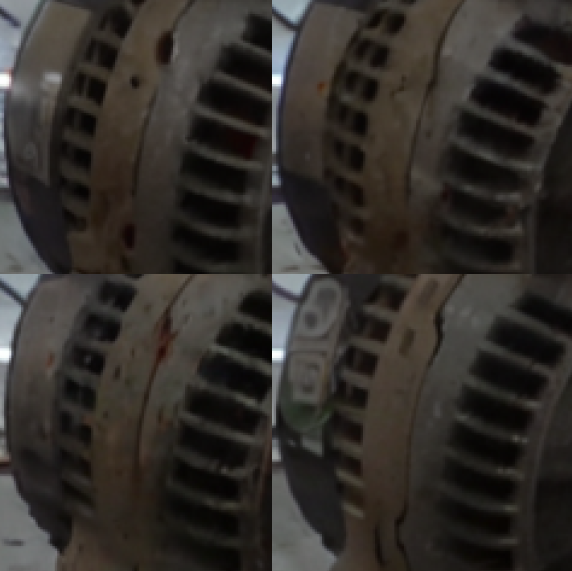
\includegraphics[width=0.48\textwidth]{figure_results_id-augs_good_1.png}%
	\hspace{0.02\textwidth}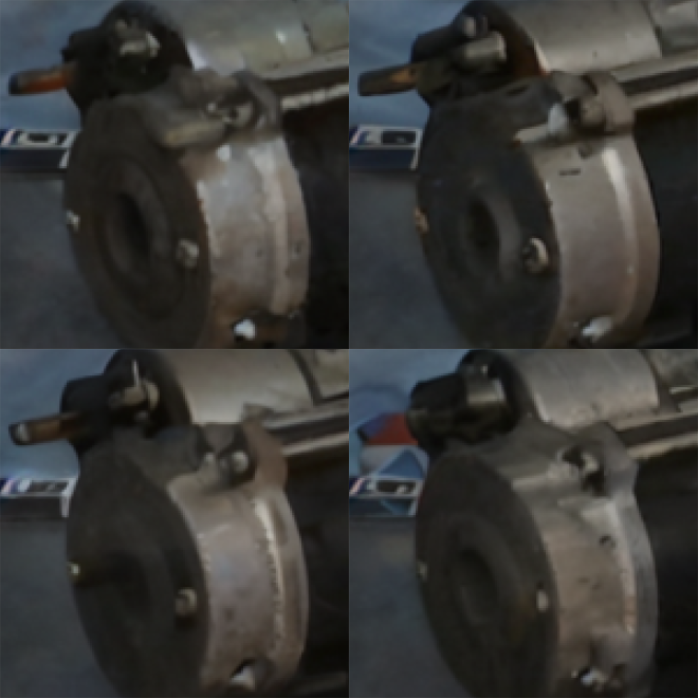
\includegraphics[width=0.48\textwidth]{figure_results_id-augs_good_2.png}
	\caption{Vergrößerte Ausschnitte von einigen der In-Distribution-Augmentationen.}
	\label{fig:id-augs-good}
\end{figure}

In einigen Fällen sind die Ergebnisse jedoch weniger überzeugend. In \autoref{fig:id-augs-bad} sind Beispiele für mangelhafte In-Distribution-Daten zu sehen. Die synthetischen Objekte sind in diesen Fällen nicht realistisch und weisen deutliche Artefakte auf. Die Qualität der Daten hängt dabei nicht nur von der Art des Objekts, sondern auch von der Größe des Objektes im Originalbild (was auch die Auflösung des ROI-Crops entscheidet). Bei glatten Oberflächen und einfachen Formen sind die Ergebnisse besser als bei komplexen Strukturen und unregelmäßigen Oberflächen.

\begin{figure}
	\centering
	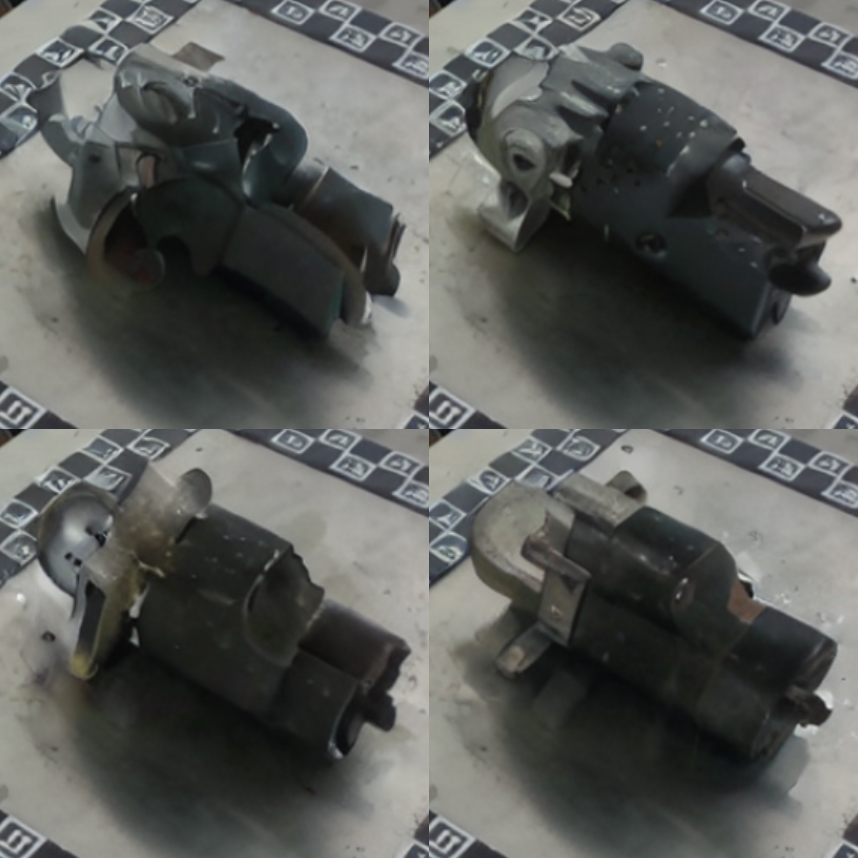
\includegraphics[width=0.48\textwidth]{figure_results_id-augs_bad_1.png}%
	\hspace{0.02\textwidth}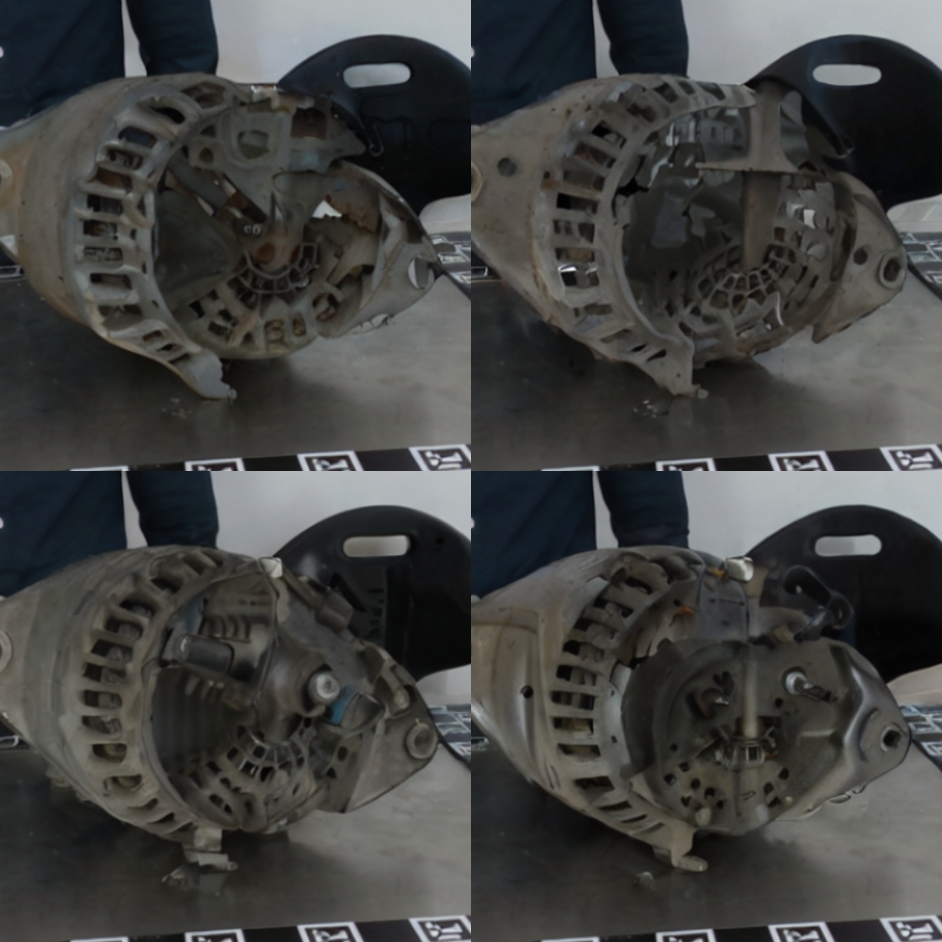
\includegraphics[width=0.48\textwidth]{figure_results_id-augs_bad_2.png}
	\caption{Beispiele für mangelhafte In-Distribution-Augmentationen.}
	\label{fig:id-augs-bad}
\end{figure}

\subsection{Near Out-of-Distribution} \label{subsec:da-fusion-ood-results}

Die synthetischen Near Out-of-Distribution-Daten sind in \autoref{fig:ood-augs-good} dargestellt. Die Qualität der Daten ist insgesamt etwas schlechter als bei den In-Distribution-Daten, was auf Grund des größeren \lstinline{strength}-Parameters von 0.5 zu erwarten war. Die Objekte wirken weniger realistisch, aber dennoch plausibel. Die Wirksamkeit der Beispiele im Training kann jedoch an dieser Stelle noch nicht beurteilt werden.

\begin{figure}
	\centering
	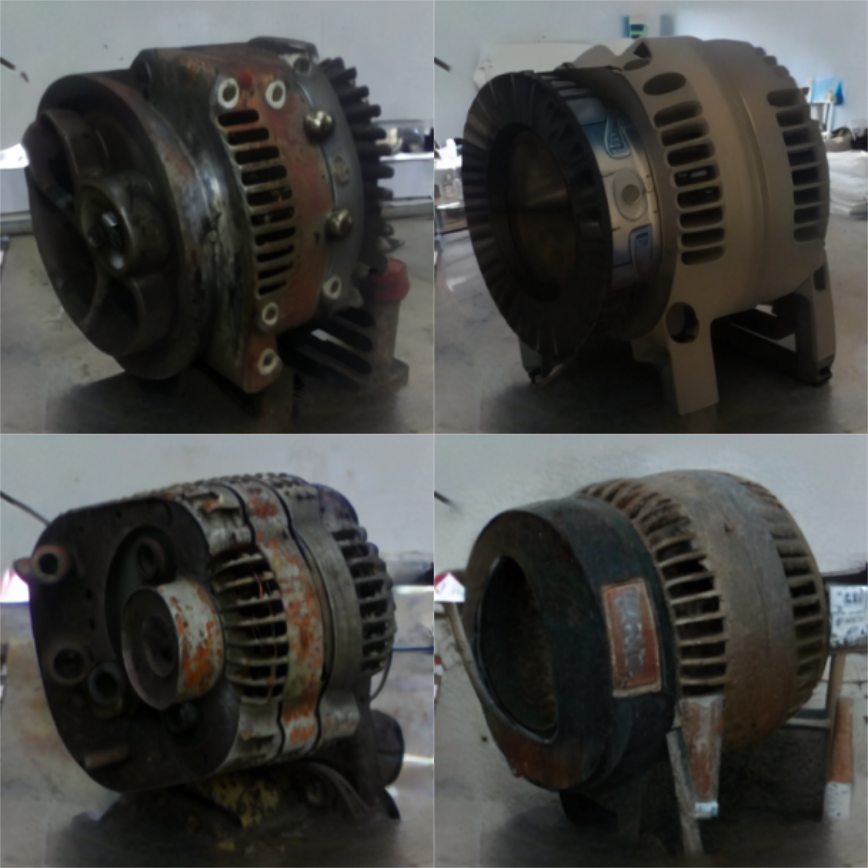
\includegraphics[width=0.48\textwidth]{figure_results_ood-augs_good_1.png}%
	\hspace{0.02\textwidth}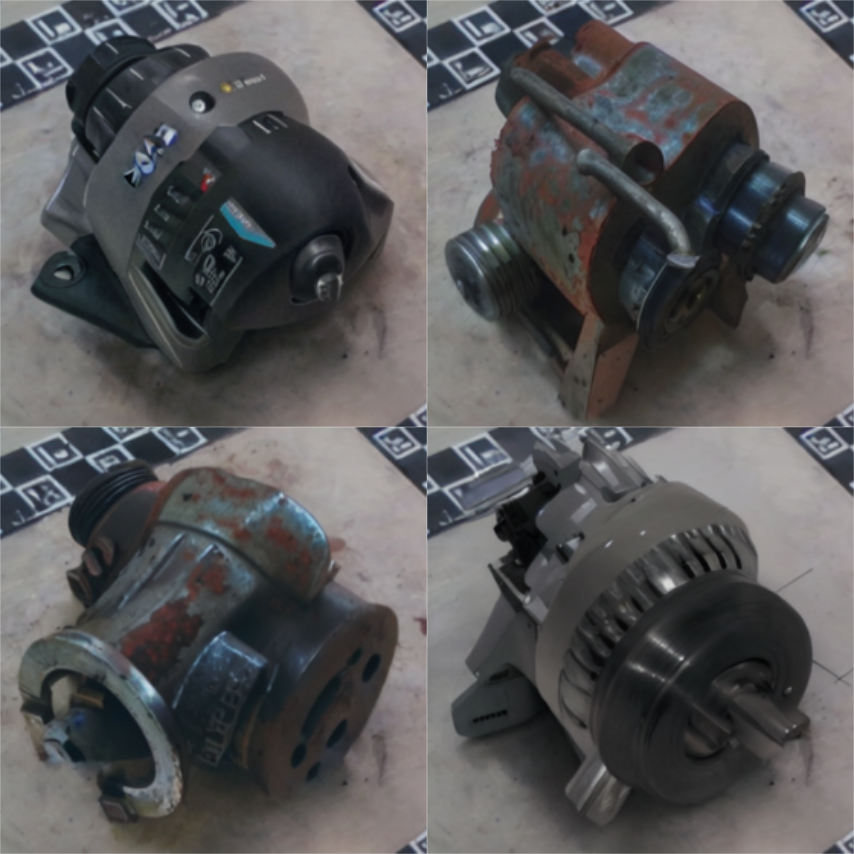
\includegraphics[width=0.48\textwidth]{figure_results_ood-augs_good_3.png}\vspace{0.01\textwidth}
	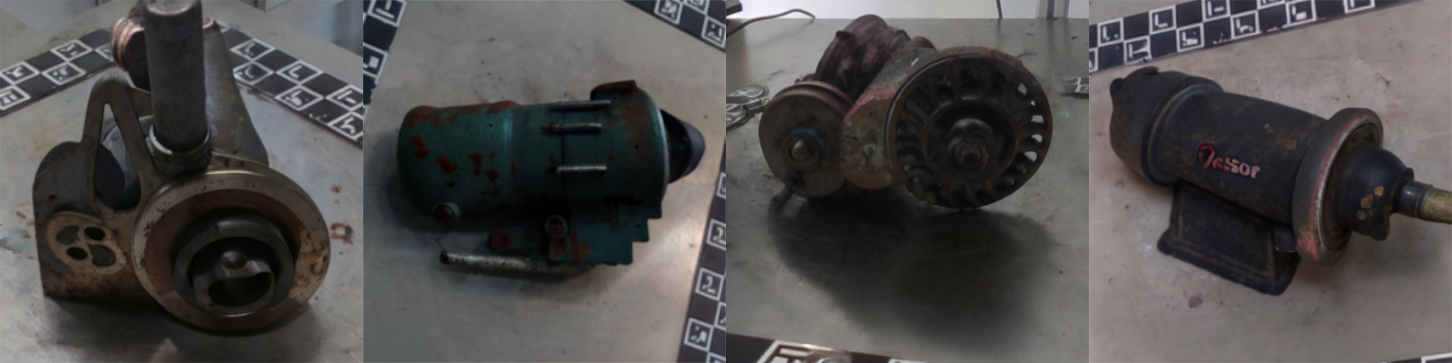
\includegraphics[width=0.98\textwidth]{figure_results_ood-augs_good_4.png}
	\caption{Beispiele der Near Out-of-Distribution-Augmentationen.}
	\label{fig:ood-augs-good}
\end{figure}

Auch hier gibt es Beispiele, die weniger überzeugend sind (siehe \autoref{fig:ood-augs-bad}). Die synthetischen Objekte weisen in diesen Fällen deutliche Artefakte auf oder sind vollständig vom ursprünglichen Konzept entkoppelt.

\begin{figure}
	\centering
	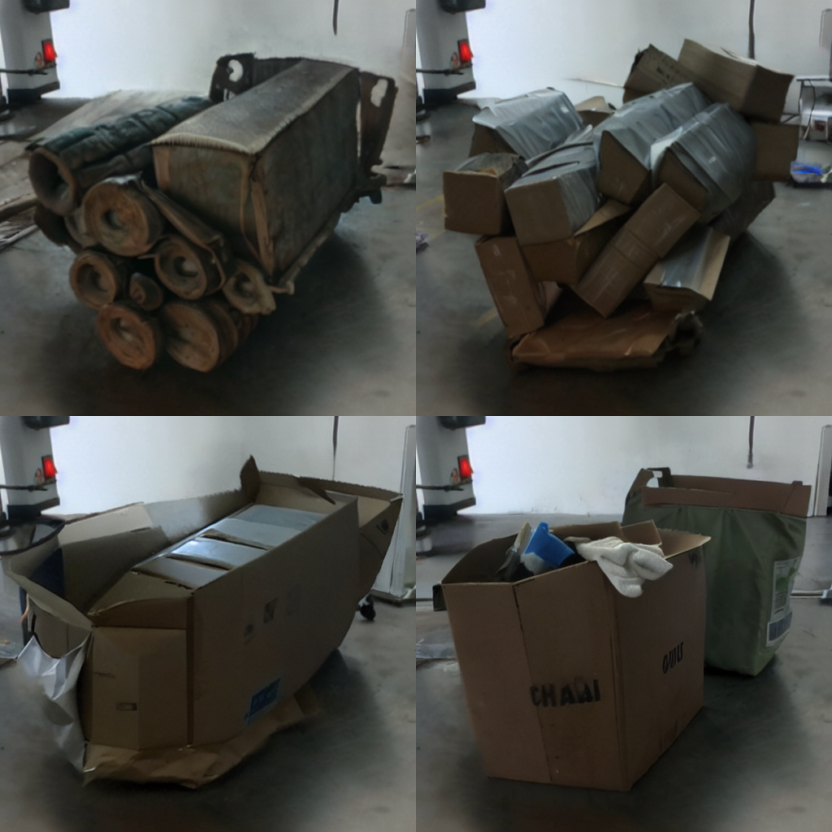
\includegraphics[width=0.48\textwidth]{figure_results_ood-augs_bad_1.png}%
	\hspace{0.02\textwidth}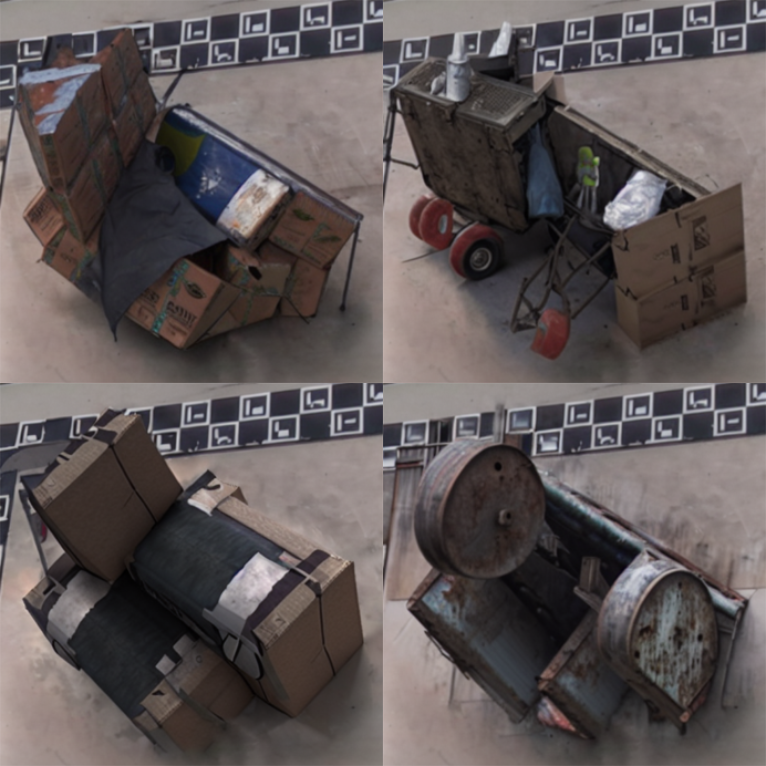
\includegraphics[width=0.48\textwidth]{figure_results_ood-augs_bad_2.png}\vspace{0.01\textwidth}
	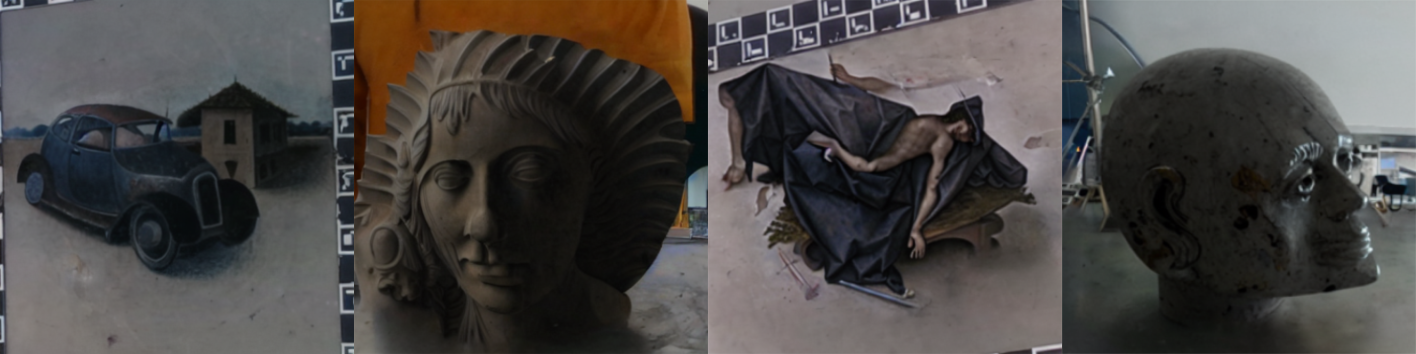
\includegraphics[width=0.98\textwidth]{figure_results_ood-augs_bad_4.png}
	\caption{Beispiele für mangelhafte Out-of-Distribution-Augmentationen.}
	\label{fig:ood-augs-bad}
\end{figure}

\section{Trainings- und Testergebnisse} \label{sec:supcon-results}

% Einleitung
Es werden nun die Ergebnisse der Trainings- und Testdurchläufe im Supervised Contrastive Learning beschrieben. Es wird auf die Trainingskurven und die Performance der Modelle eingegangen.

\subsection{Contrastive Pre-Training} \label{subsec:supcon-pre-results}

\autoref{fig:supcon-pre-loss} zeigt die Trainingskurven des Contrastive Pre-Trainings. Die Trainings- und Validierungsfehler zeigen insgesamt eine gute Konvergenz, wobei zu erkennen ist, dass der Validierungsfehler im Vergleich zum Trainingsfehler etwas höher und weniger stabil ist.

\begin{figure}[h]
	\centering
	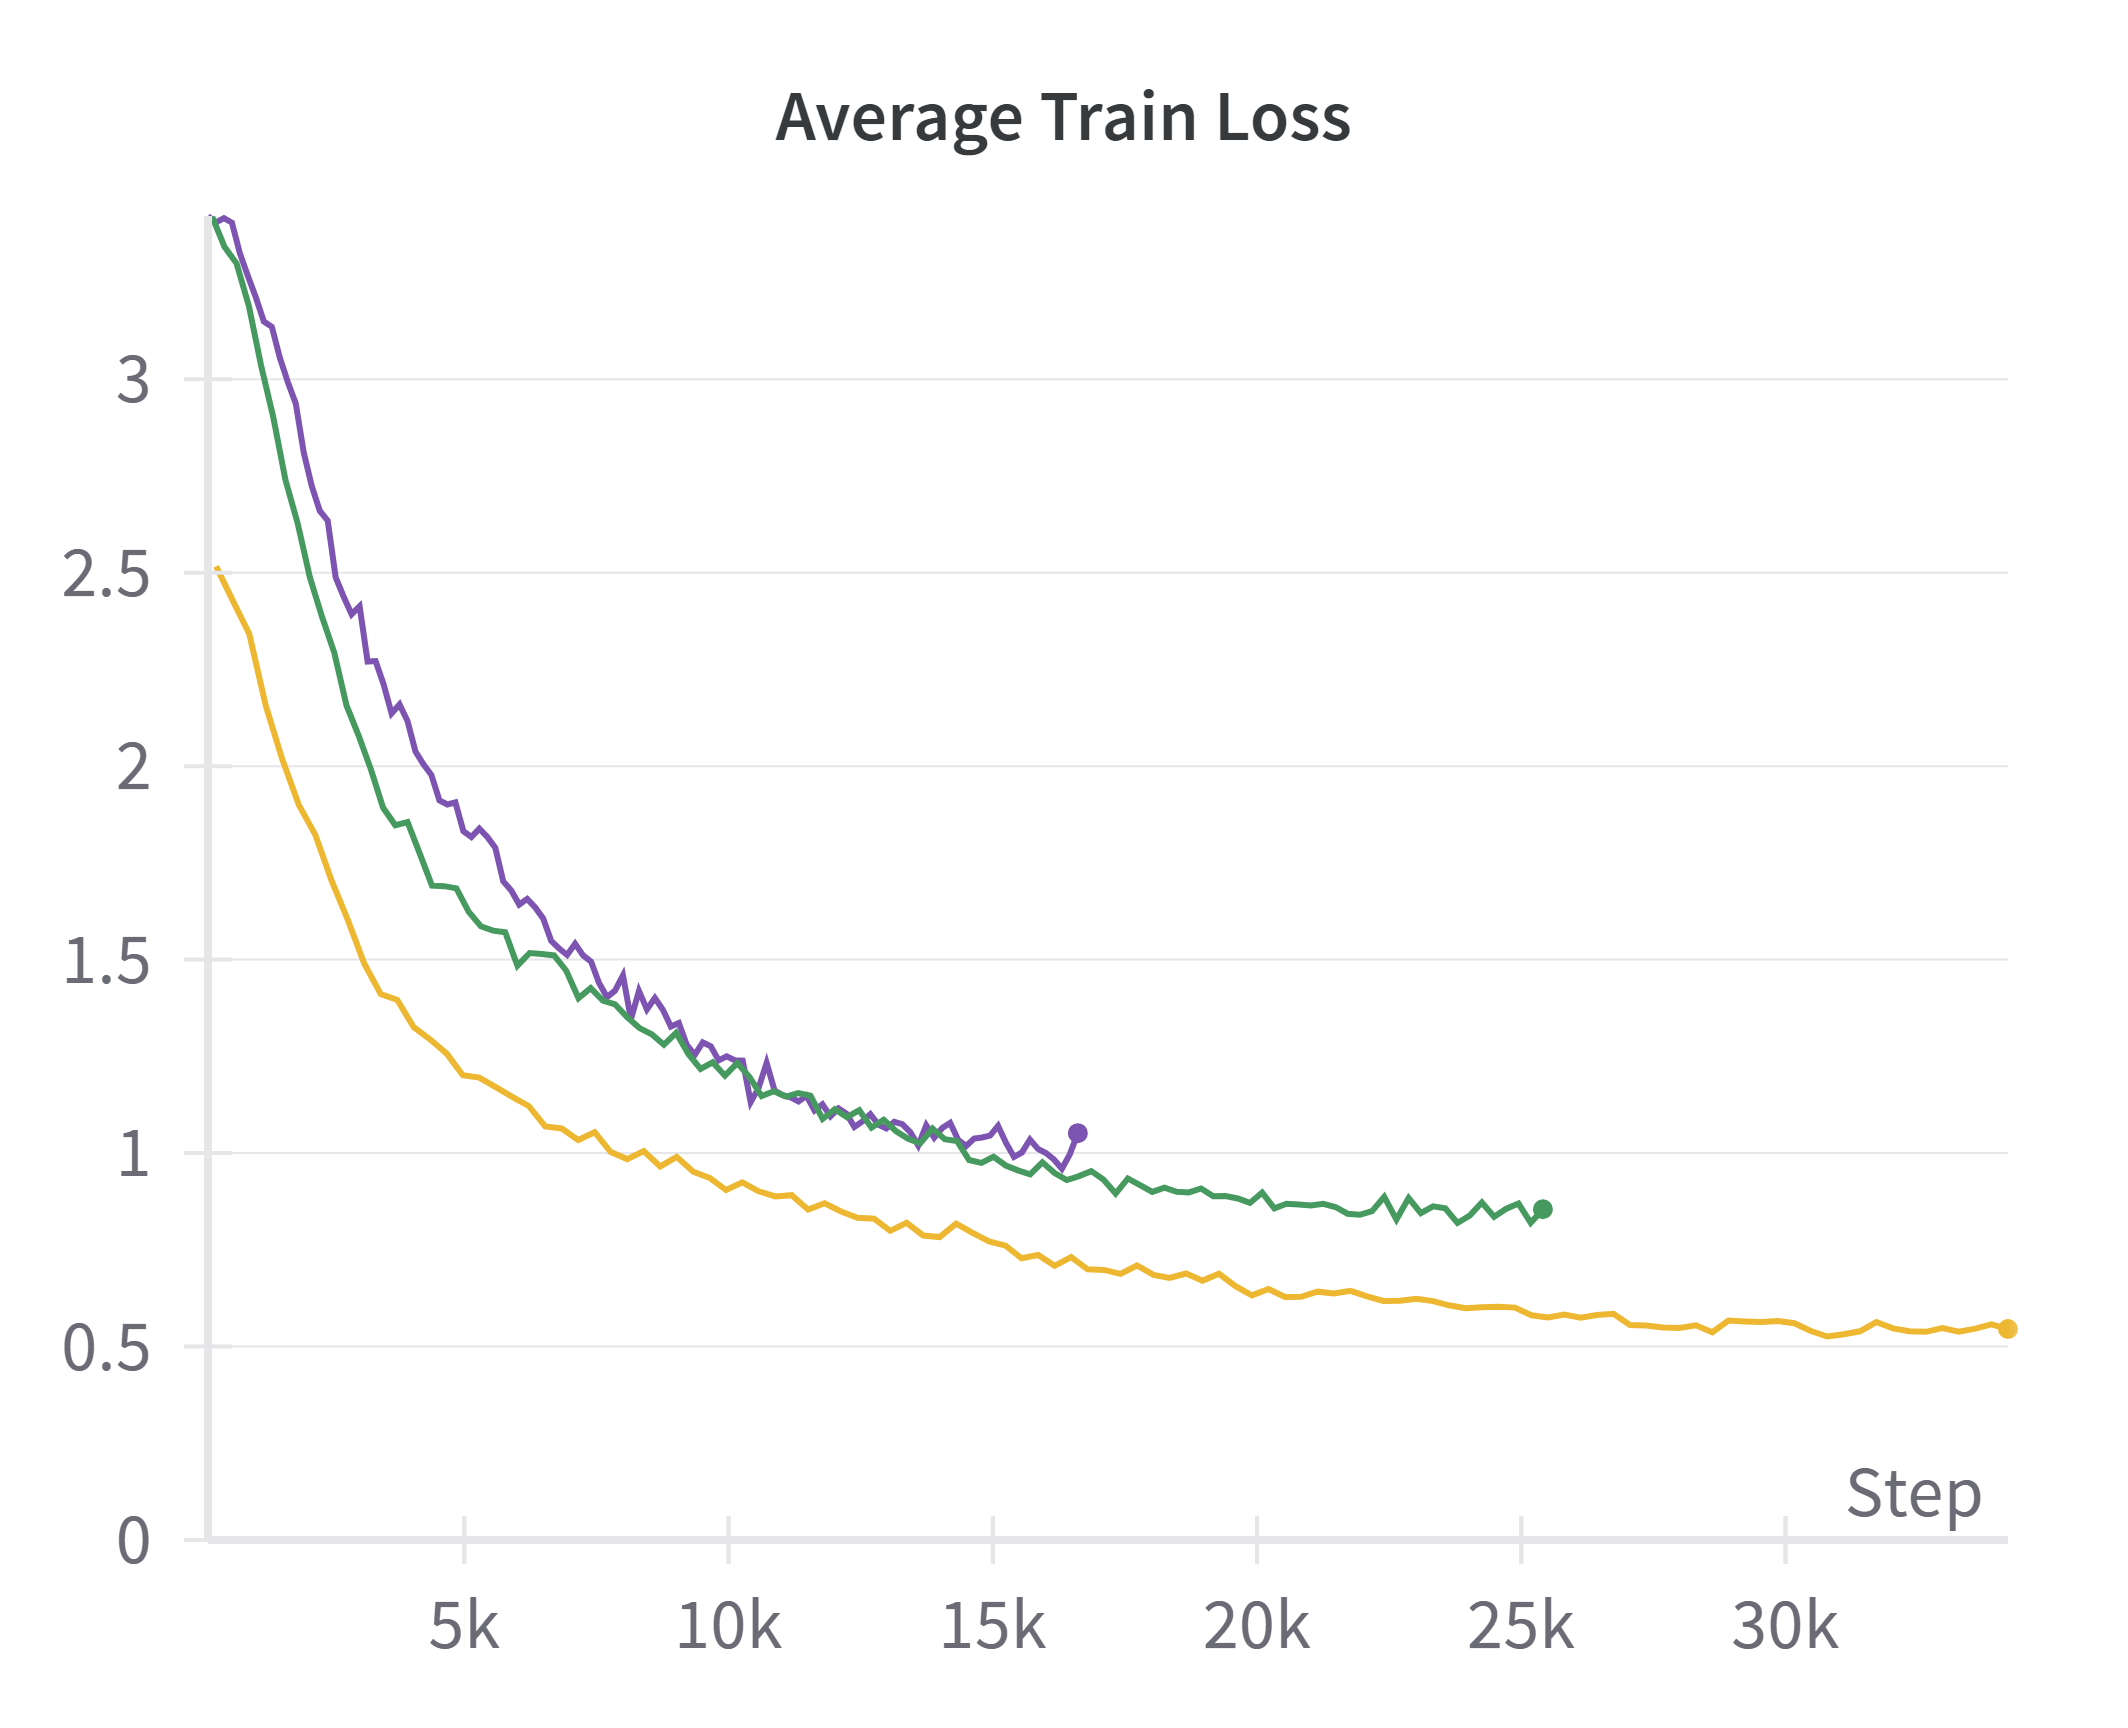
\includegraphics[width=0.5\textwidth]{figure_results_supcon-pre_avg-train-loss.png}%
	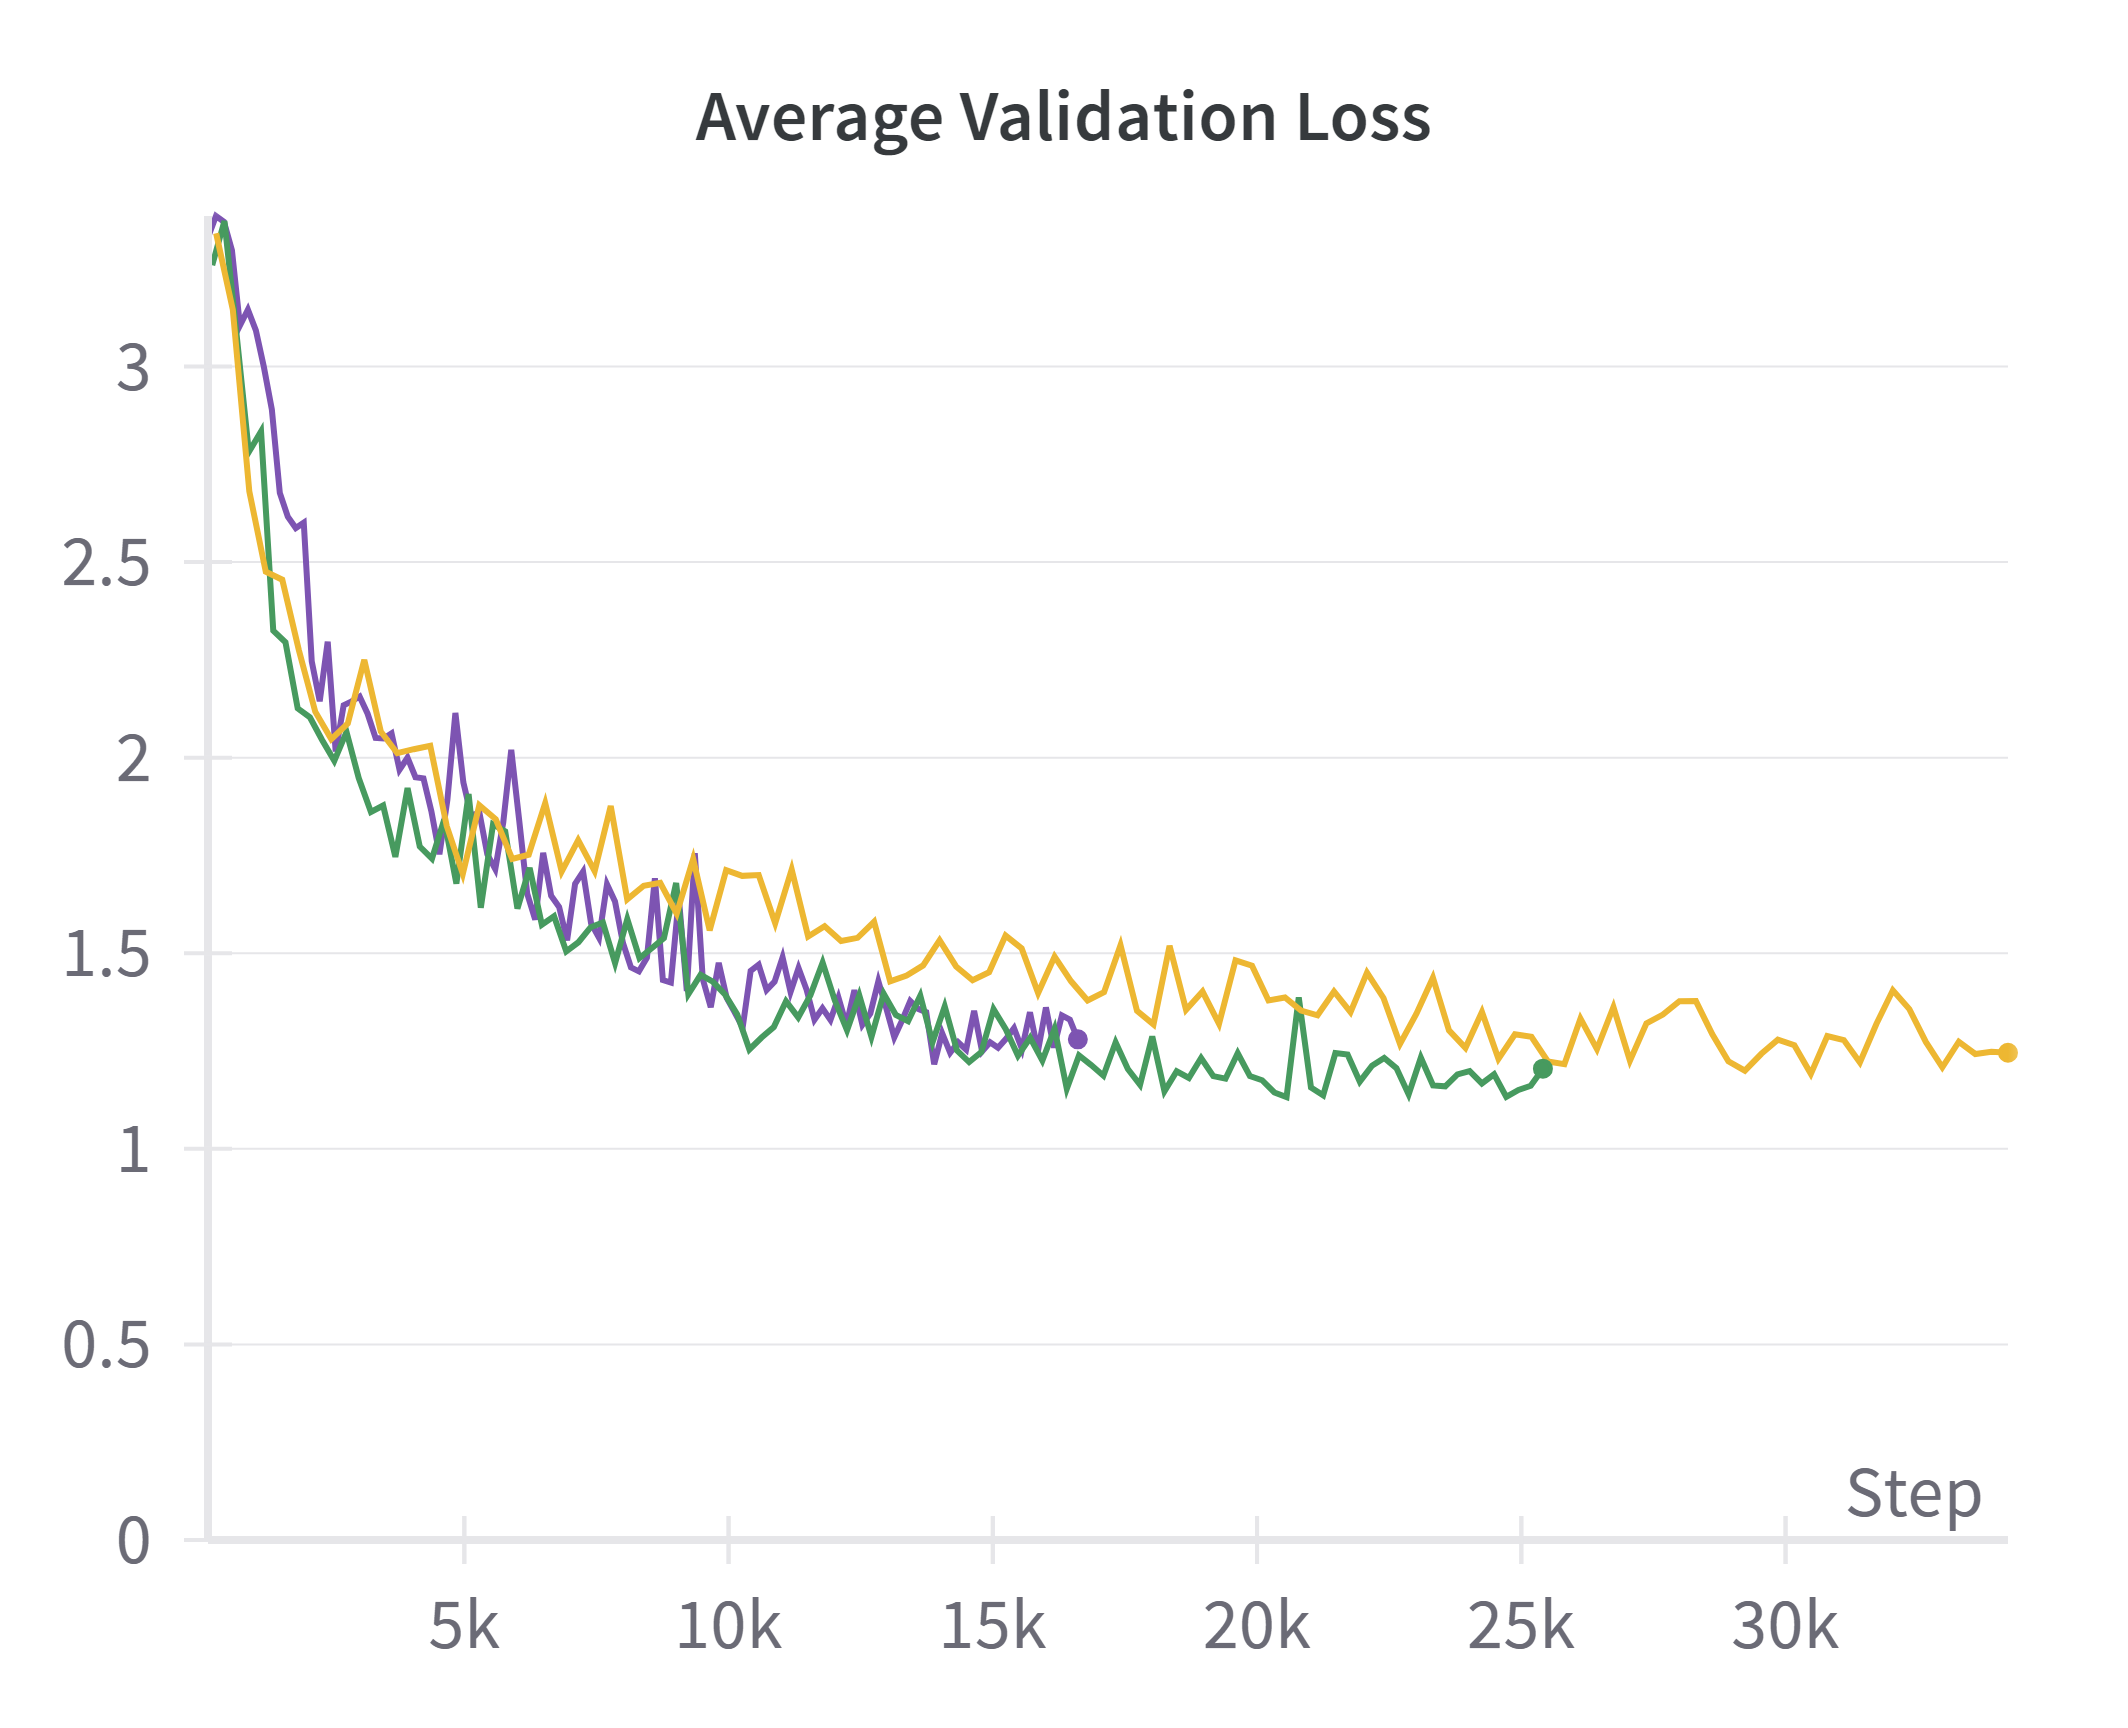
\includegraphics[width=0.5\textwidth]{figure_results_supcon-pre_avg-val-loss.png}
	\caption[Trainings- und Validierungsfehler während des Contrastive Pre-Trainings.]{Trainings- und Validierungsfehler während des Contrastive Pre-Trainings (\textcolor{exp1}{Lila}: Versuch 1, \textcolor{exp2}{Grün}: Versuch 2, \textcolor{exp3}{Gelb}: Versuch 3).}
	\label{fig:supcon-pre-loss}
\end{figure}

% Leichte Verbesserung bei Versuch 2
Der Fehler auf den Trainings- und Validierungsdaten verläuft bei Versuch 2 fast identisch zu Versuch 1, durch die zusätzlichen Augmentationen läuft das Training jedoch ein wenig länger, sodass die Performance sich weiter verbessert.

% Leichte Verschlechterung bei Versuch 3
Versuch 3 zeigt auf den Trainingsdaten einen insgesamt deutlich niedrigeren Fehler, während der Fehler auf den Validierungsdaten bis zum Ende des Trainings etwas höher ist als bei den anderen Versuchen, trotz der längsten Trainingsdauer.

\subsection{Lineare Klassifikation} \label{subsec:supcon-lin-results}

Die Trainingskurven der linearen Klassifikation sind in \autoref{fig:supcon-lin-loss-acc} (Fehler und Accuracy) und \autoref{fig:supcon-lin-ood-detection} (ID- und OOD-Confidence) zu sehen.

In allen Versuchen zeigt sich eine gute Konvergenz der Trainings- und Validierungskurven. Die Trainings- und Validierungsfehler sind dabei sehr niedrig und stabil, wobei der Validierungsfehler im Vergleich zum Trainingsfehler etwas höher ist. Die Trainings- und Validierungsgenauigkeiten sind ebenfalls sehr hoch und stabil, wobei die Validierungsgenauigkeit im Vergleich zur Trainingsgenauigkeit etwas niedriger ist. Die ID- und OOD-Confidence sind ebenfalls relativ hoch, es gibt jedoch einen klaren Abstand zwischen ID-Confidence und OOD-Confidence.

\begin{figure}
	\centering
	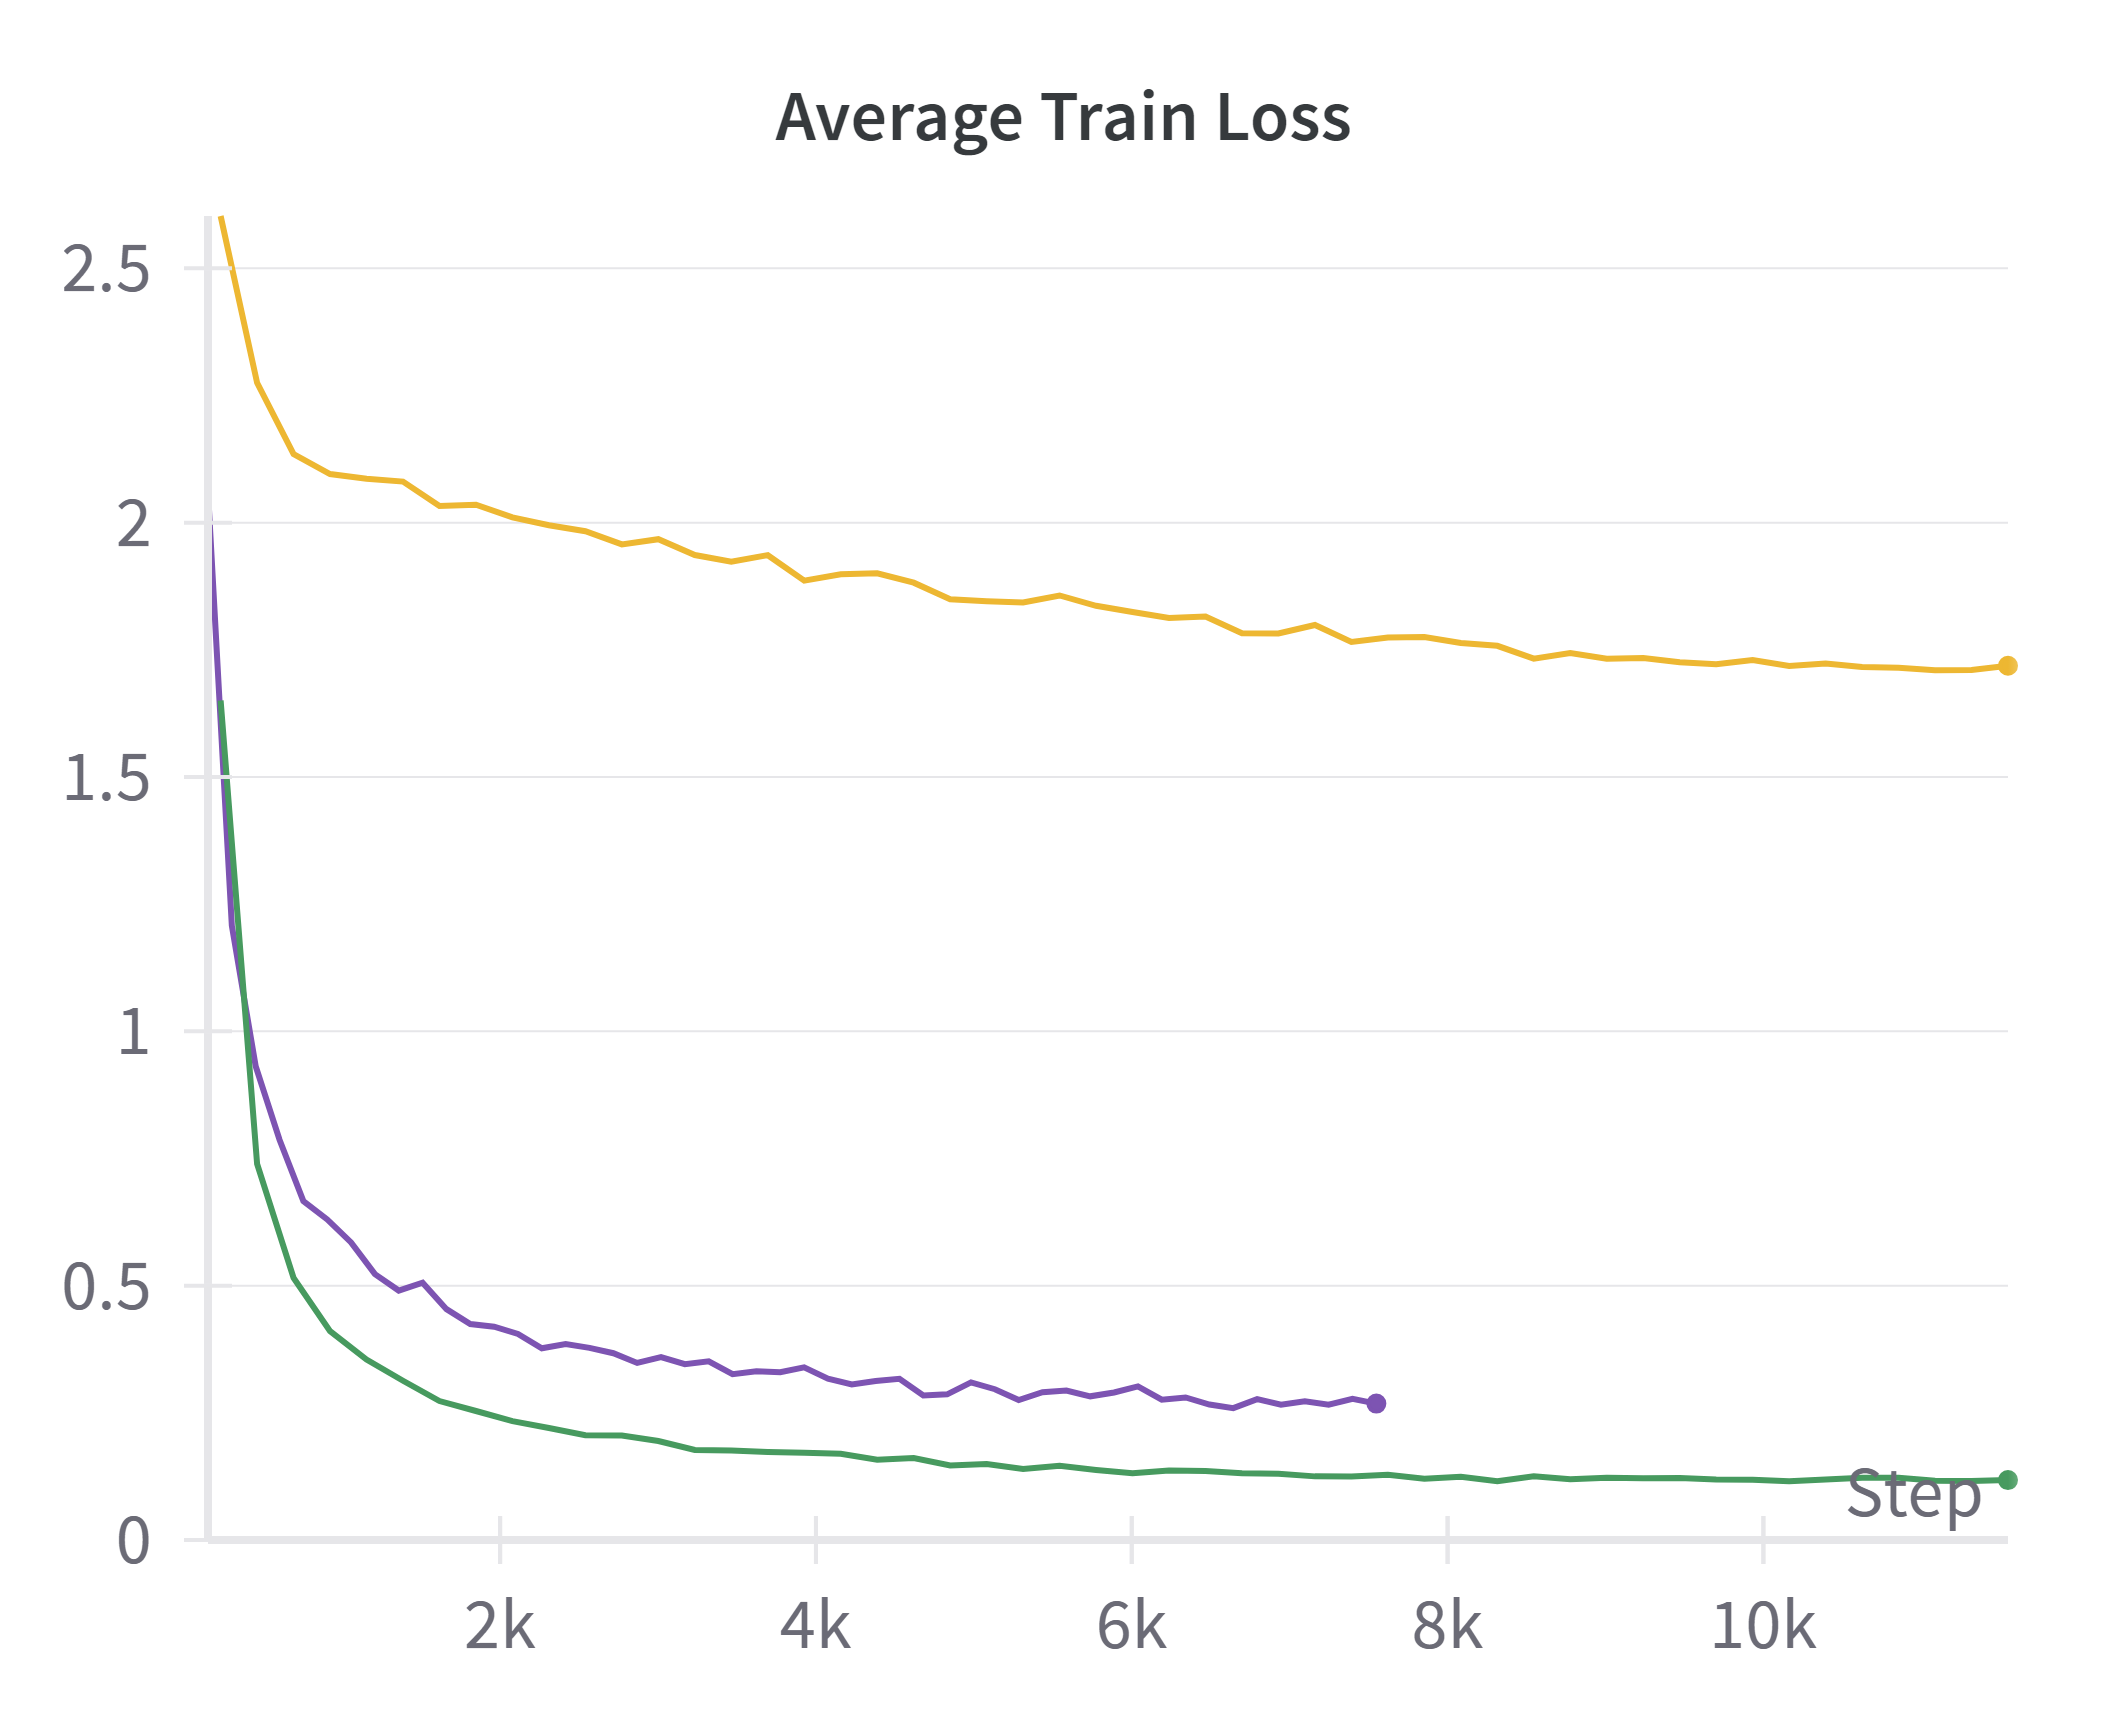
\includegraphics[width=0.5\textwidth]{figure_results_supcon-lin_avg-train-loss.png}%
	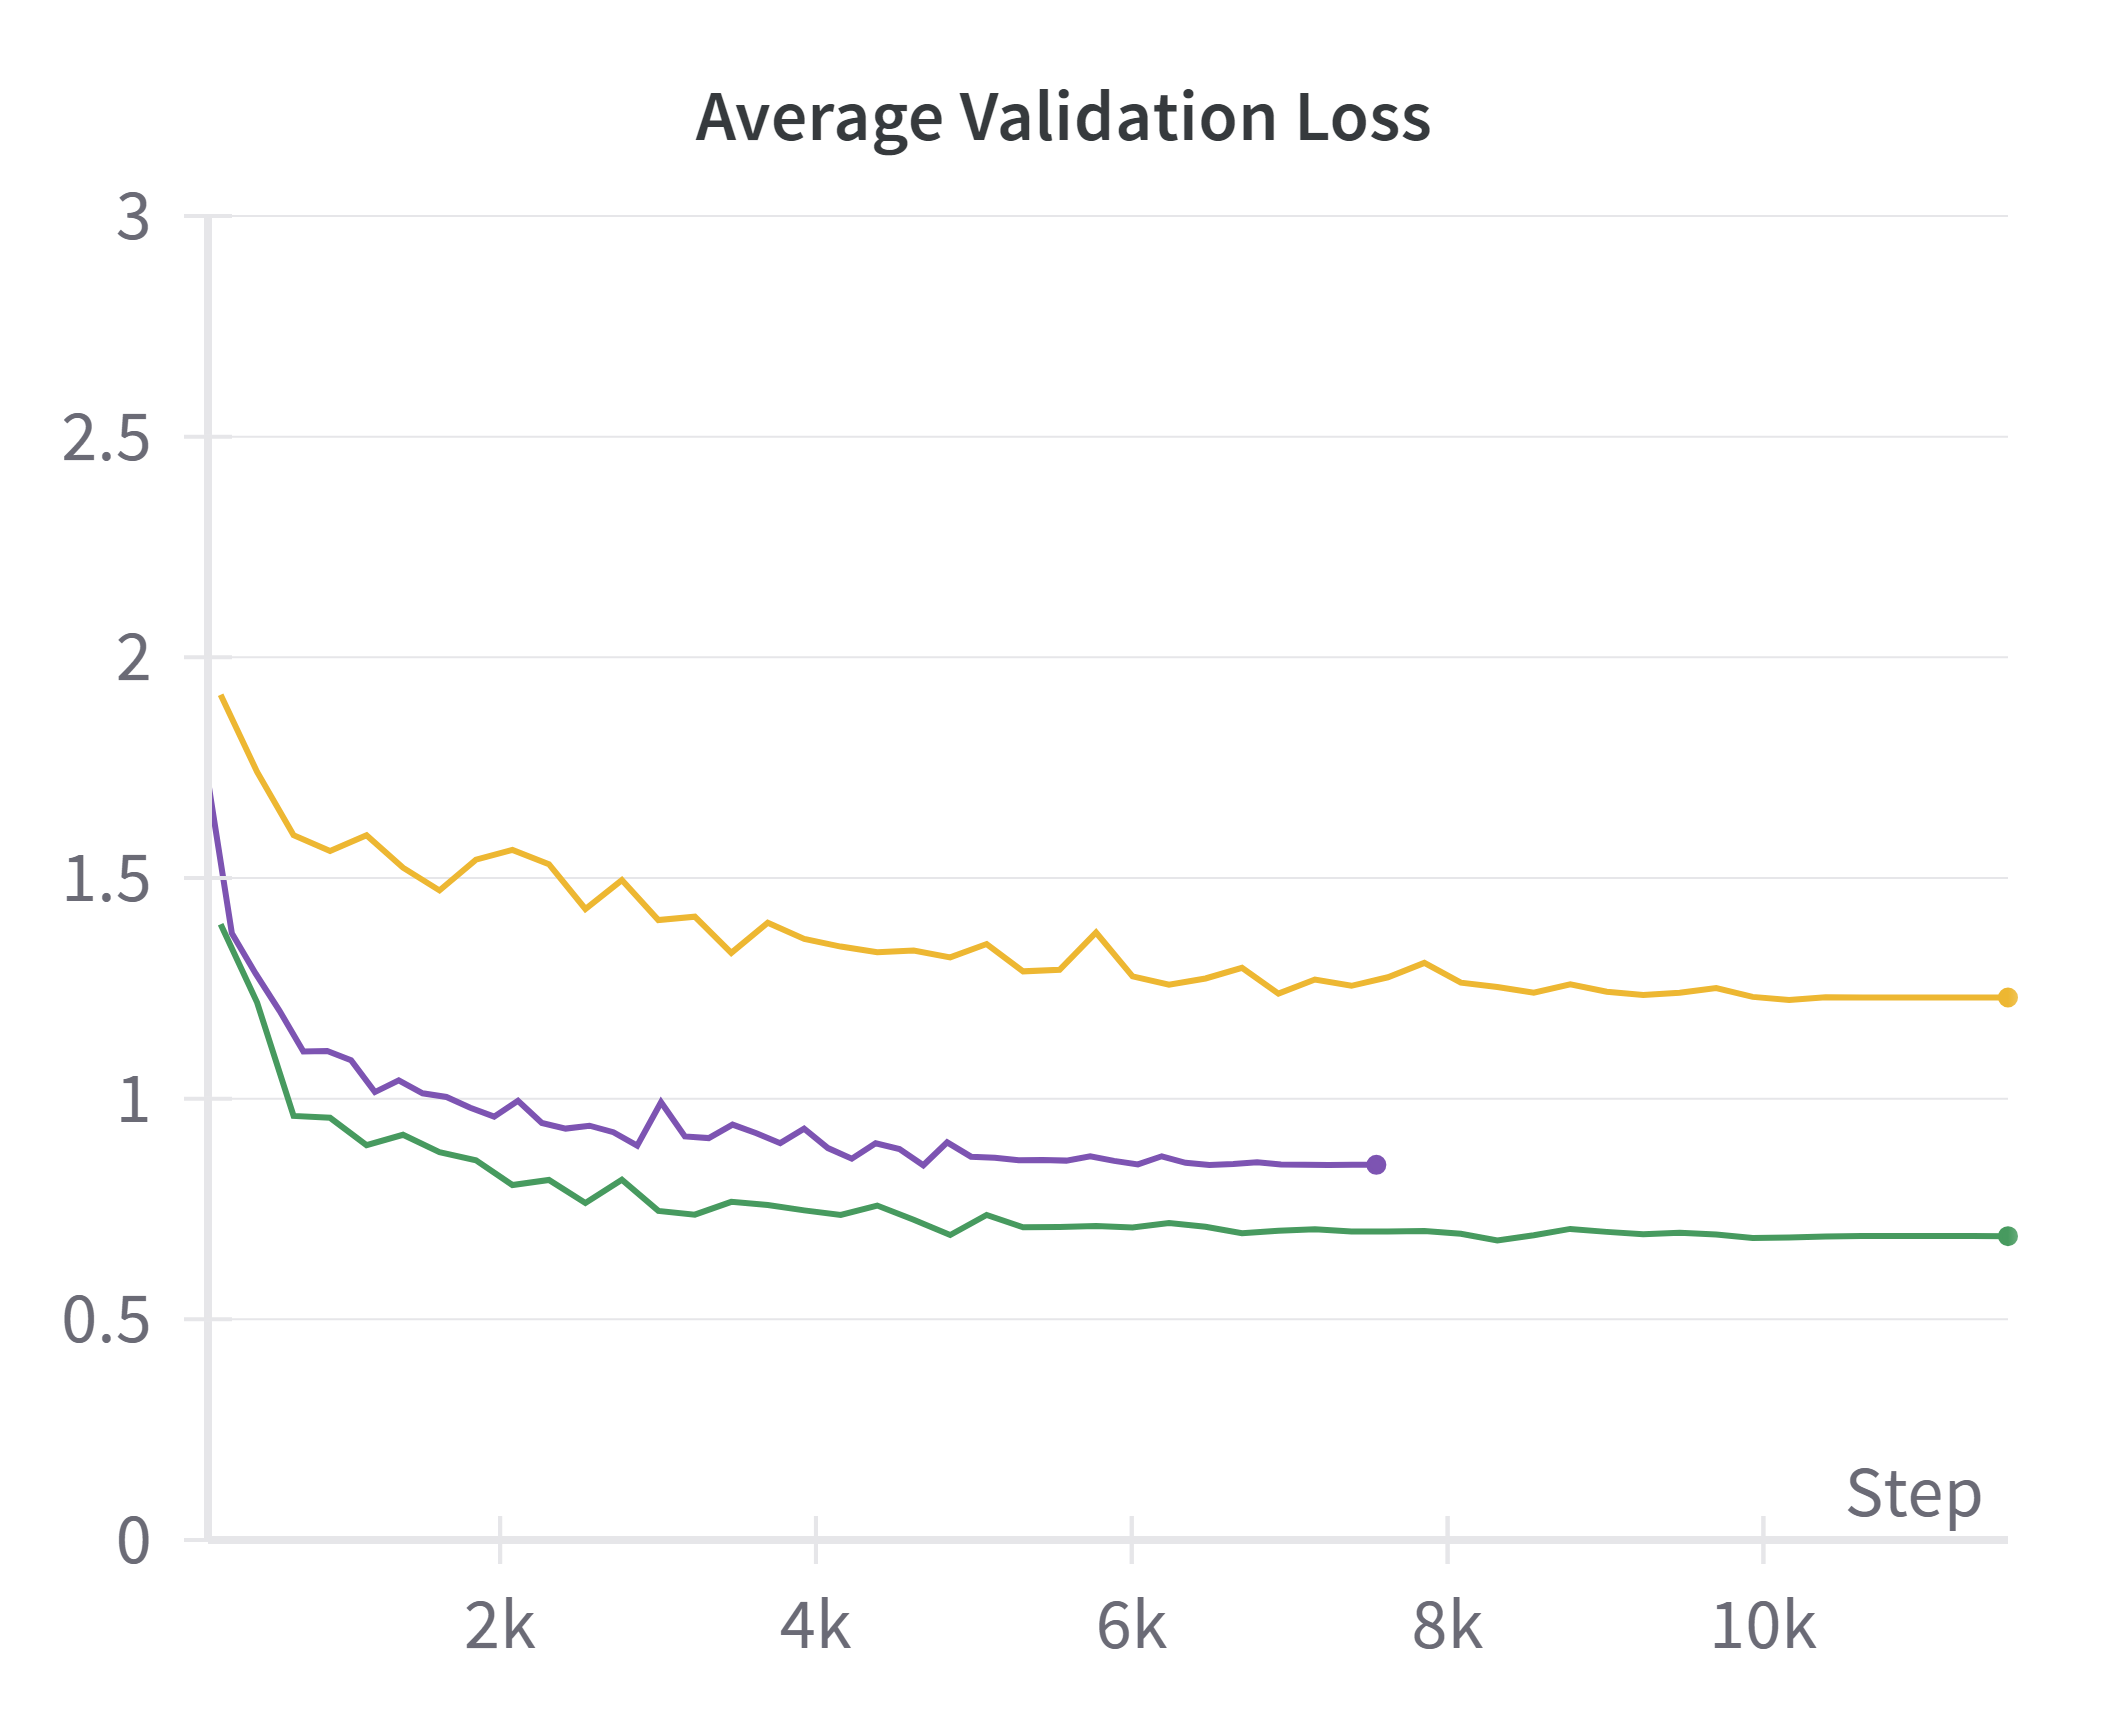
\includegraphics[width=0.5\textwidth]{figure_results_supcon-lin_avg-val-loss.png}
	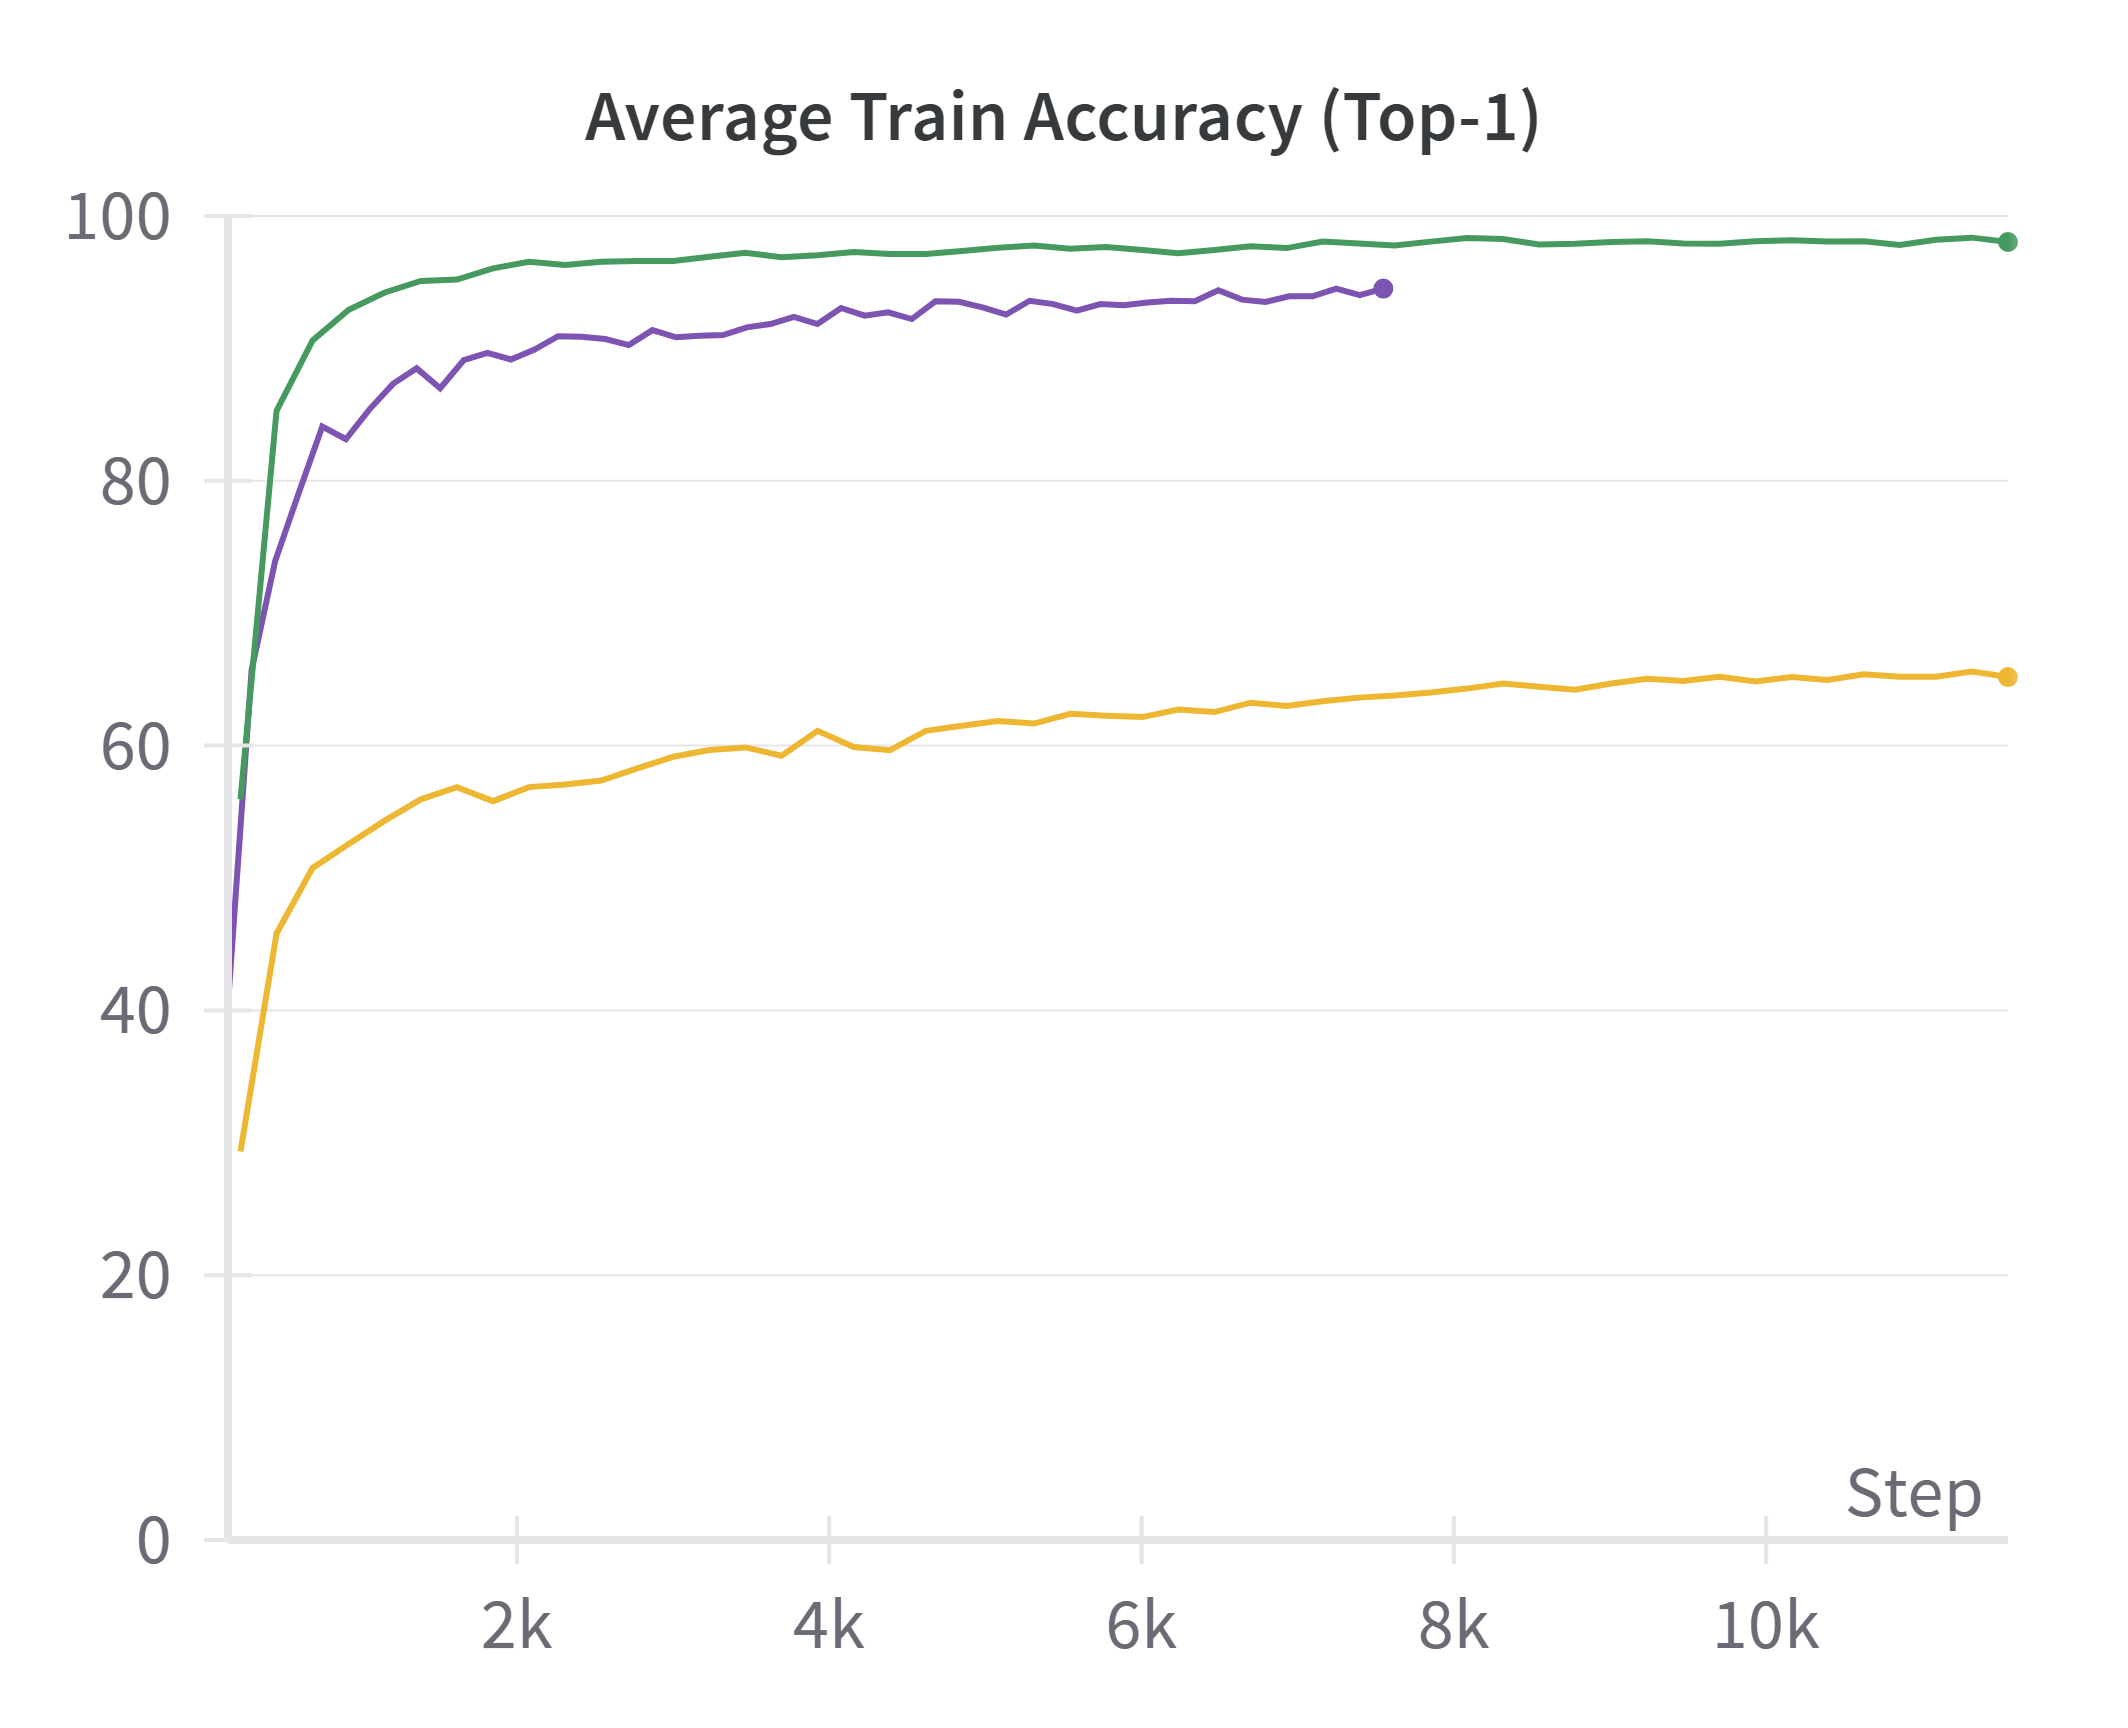
\includegraphics[width=0.5\textwidth]{figure_results_supcon-lin_avg-train-acc.png}%
	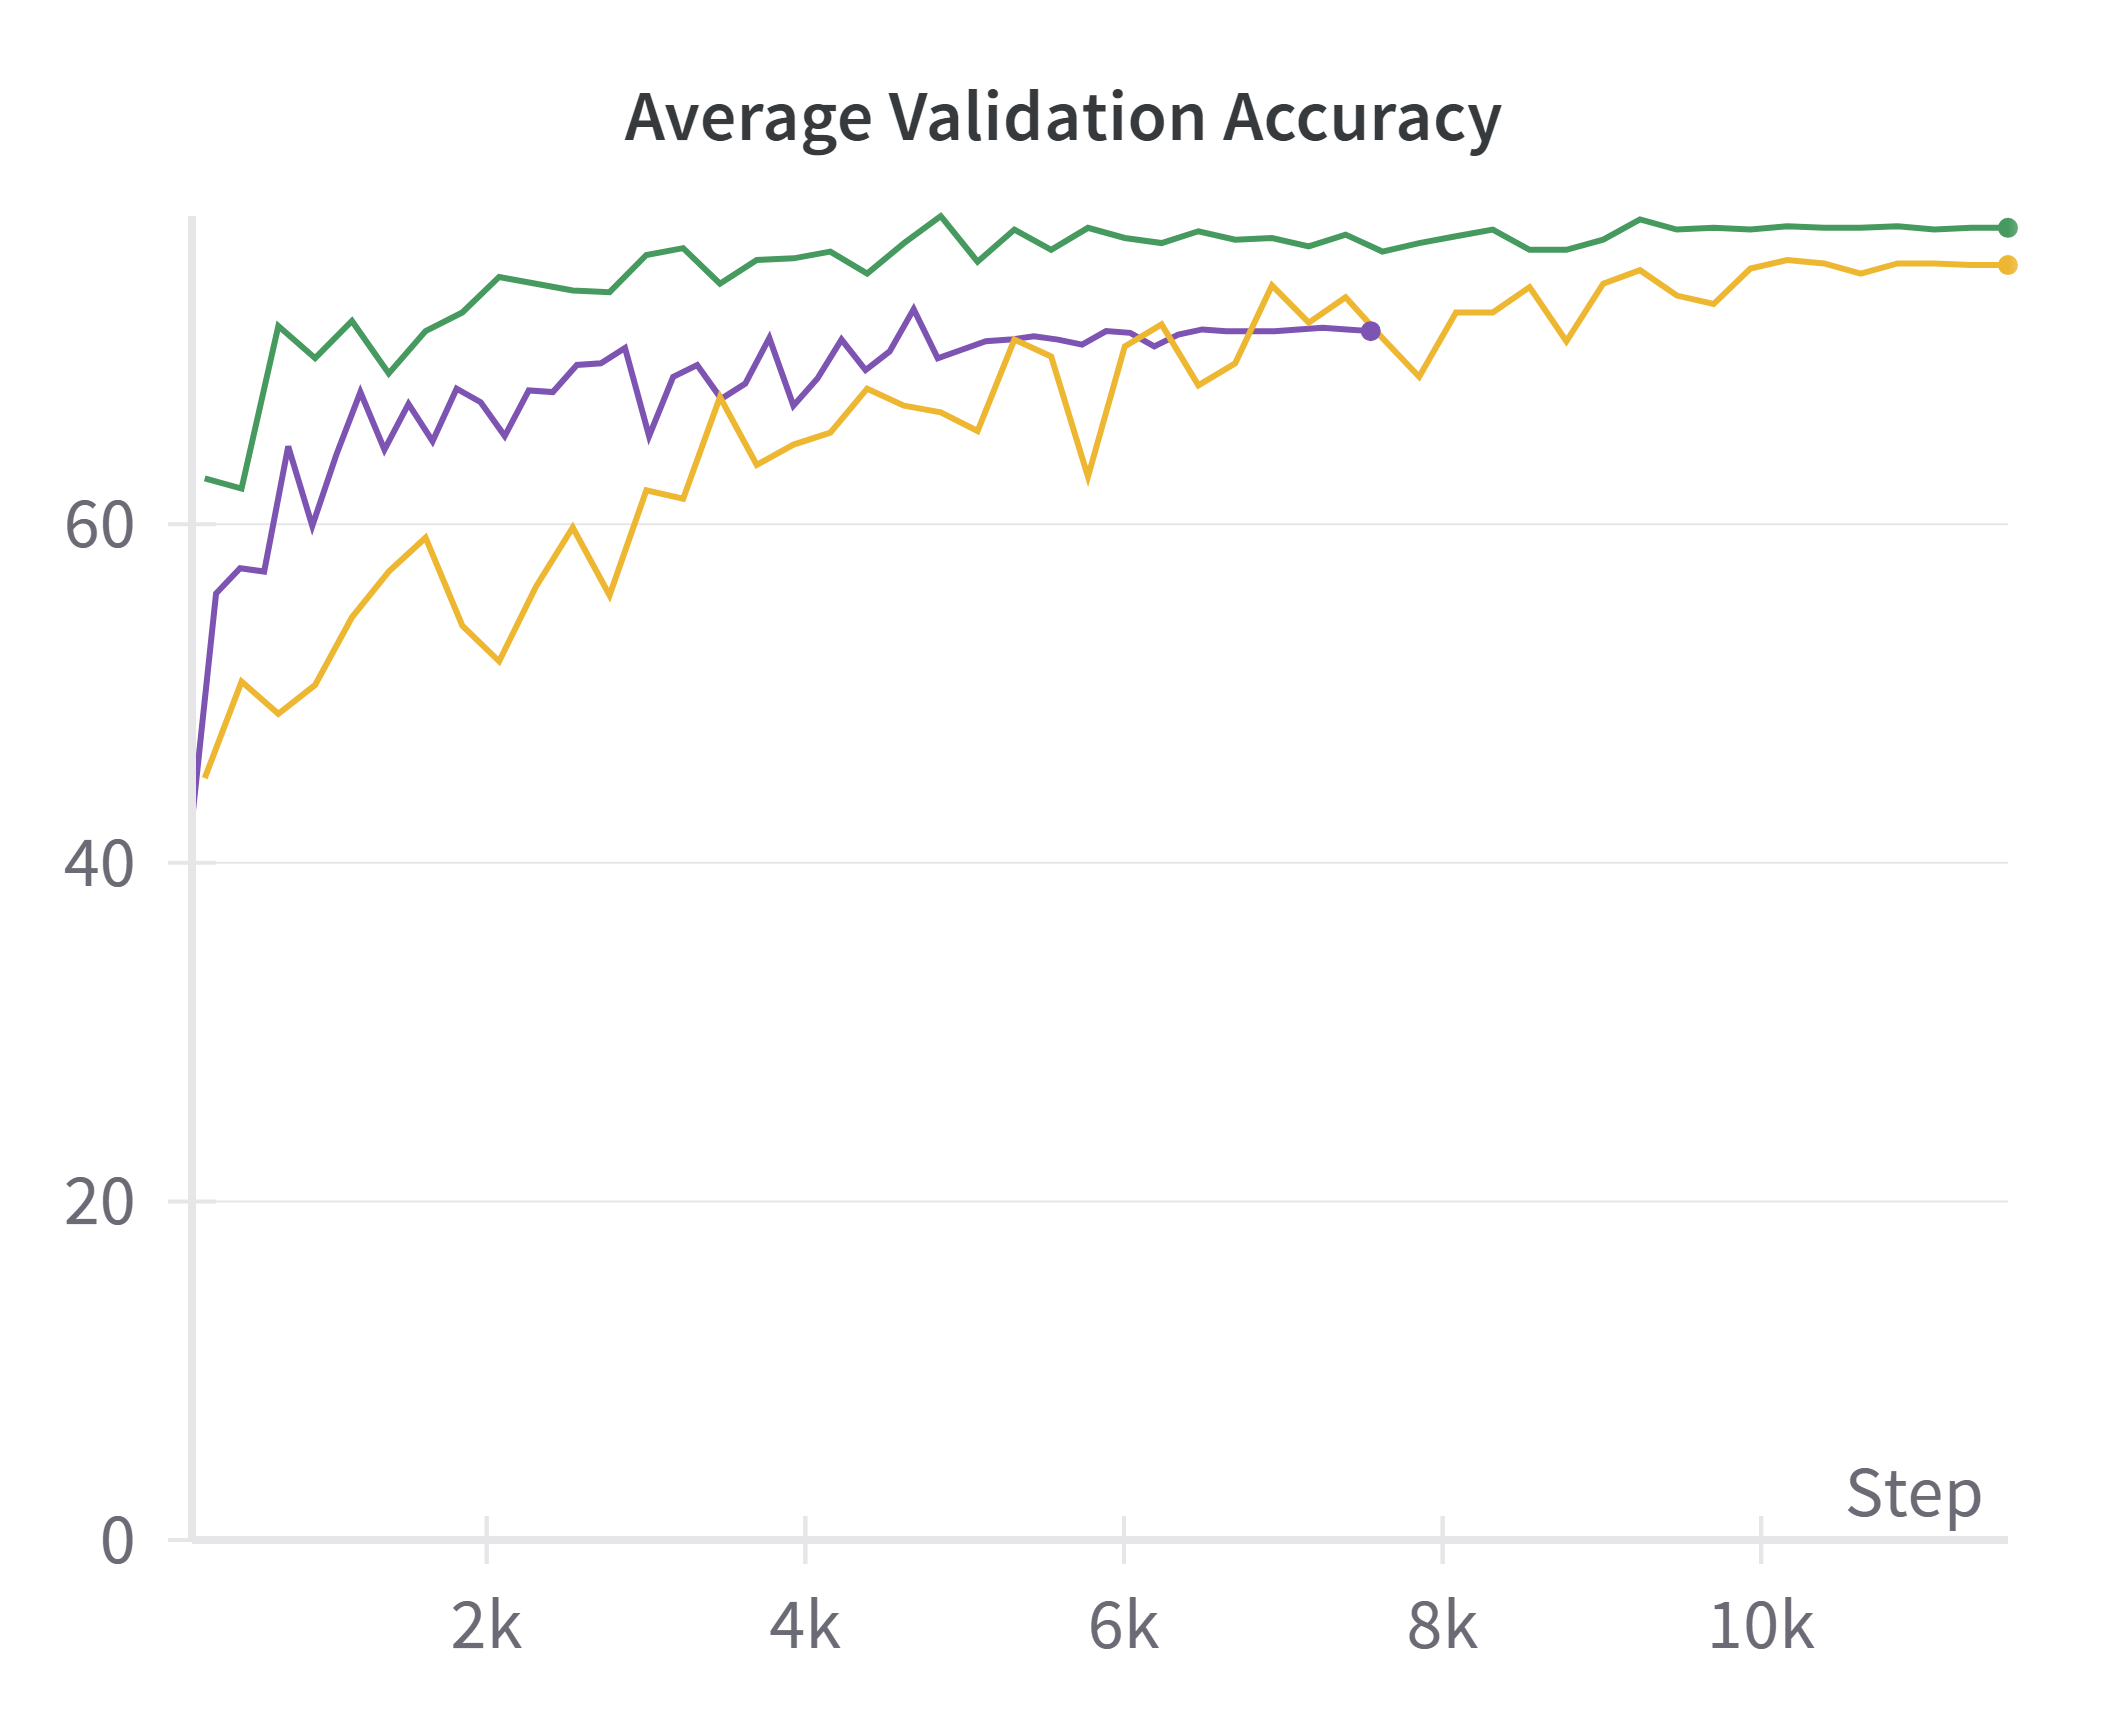
\includegraphics[width=0.5\textwidth]{figure_results_supcon-lin_avg-val-acc.png}
	\caption[Trainings- und Validierungsfehler bzw. -Accuracy während der linearen Klassifikation.]{Trainings- und Validierungsfehler bzw. -Accuracy während der linearen Klassifikation. \textcolor{exp1}{Lila}: Versuch 1, \textcolor{exp2}{Grün}: Versuch 2, \textcolor{exp3}{Gelb}: Versuch 3.}
	\label{fig:supcon-lin-loss-acc}
\end{figure}
\begin{figure}[]
	\centering
	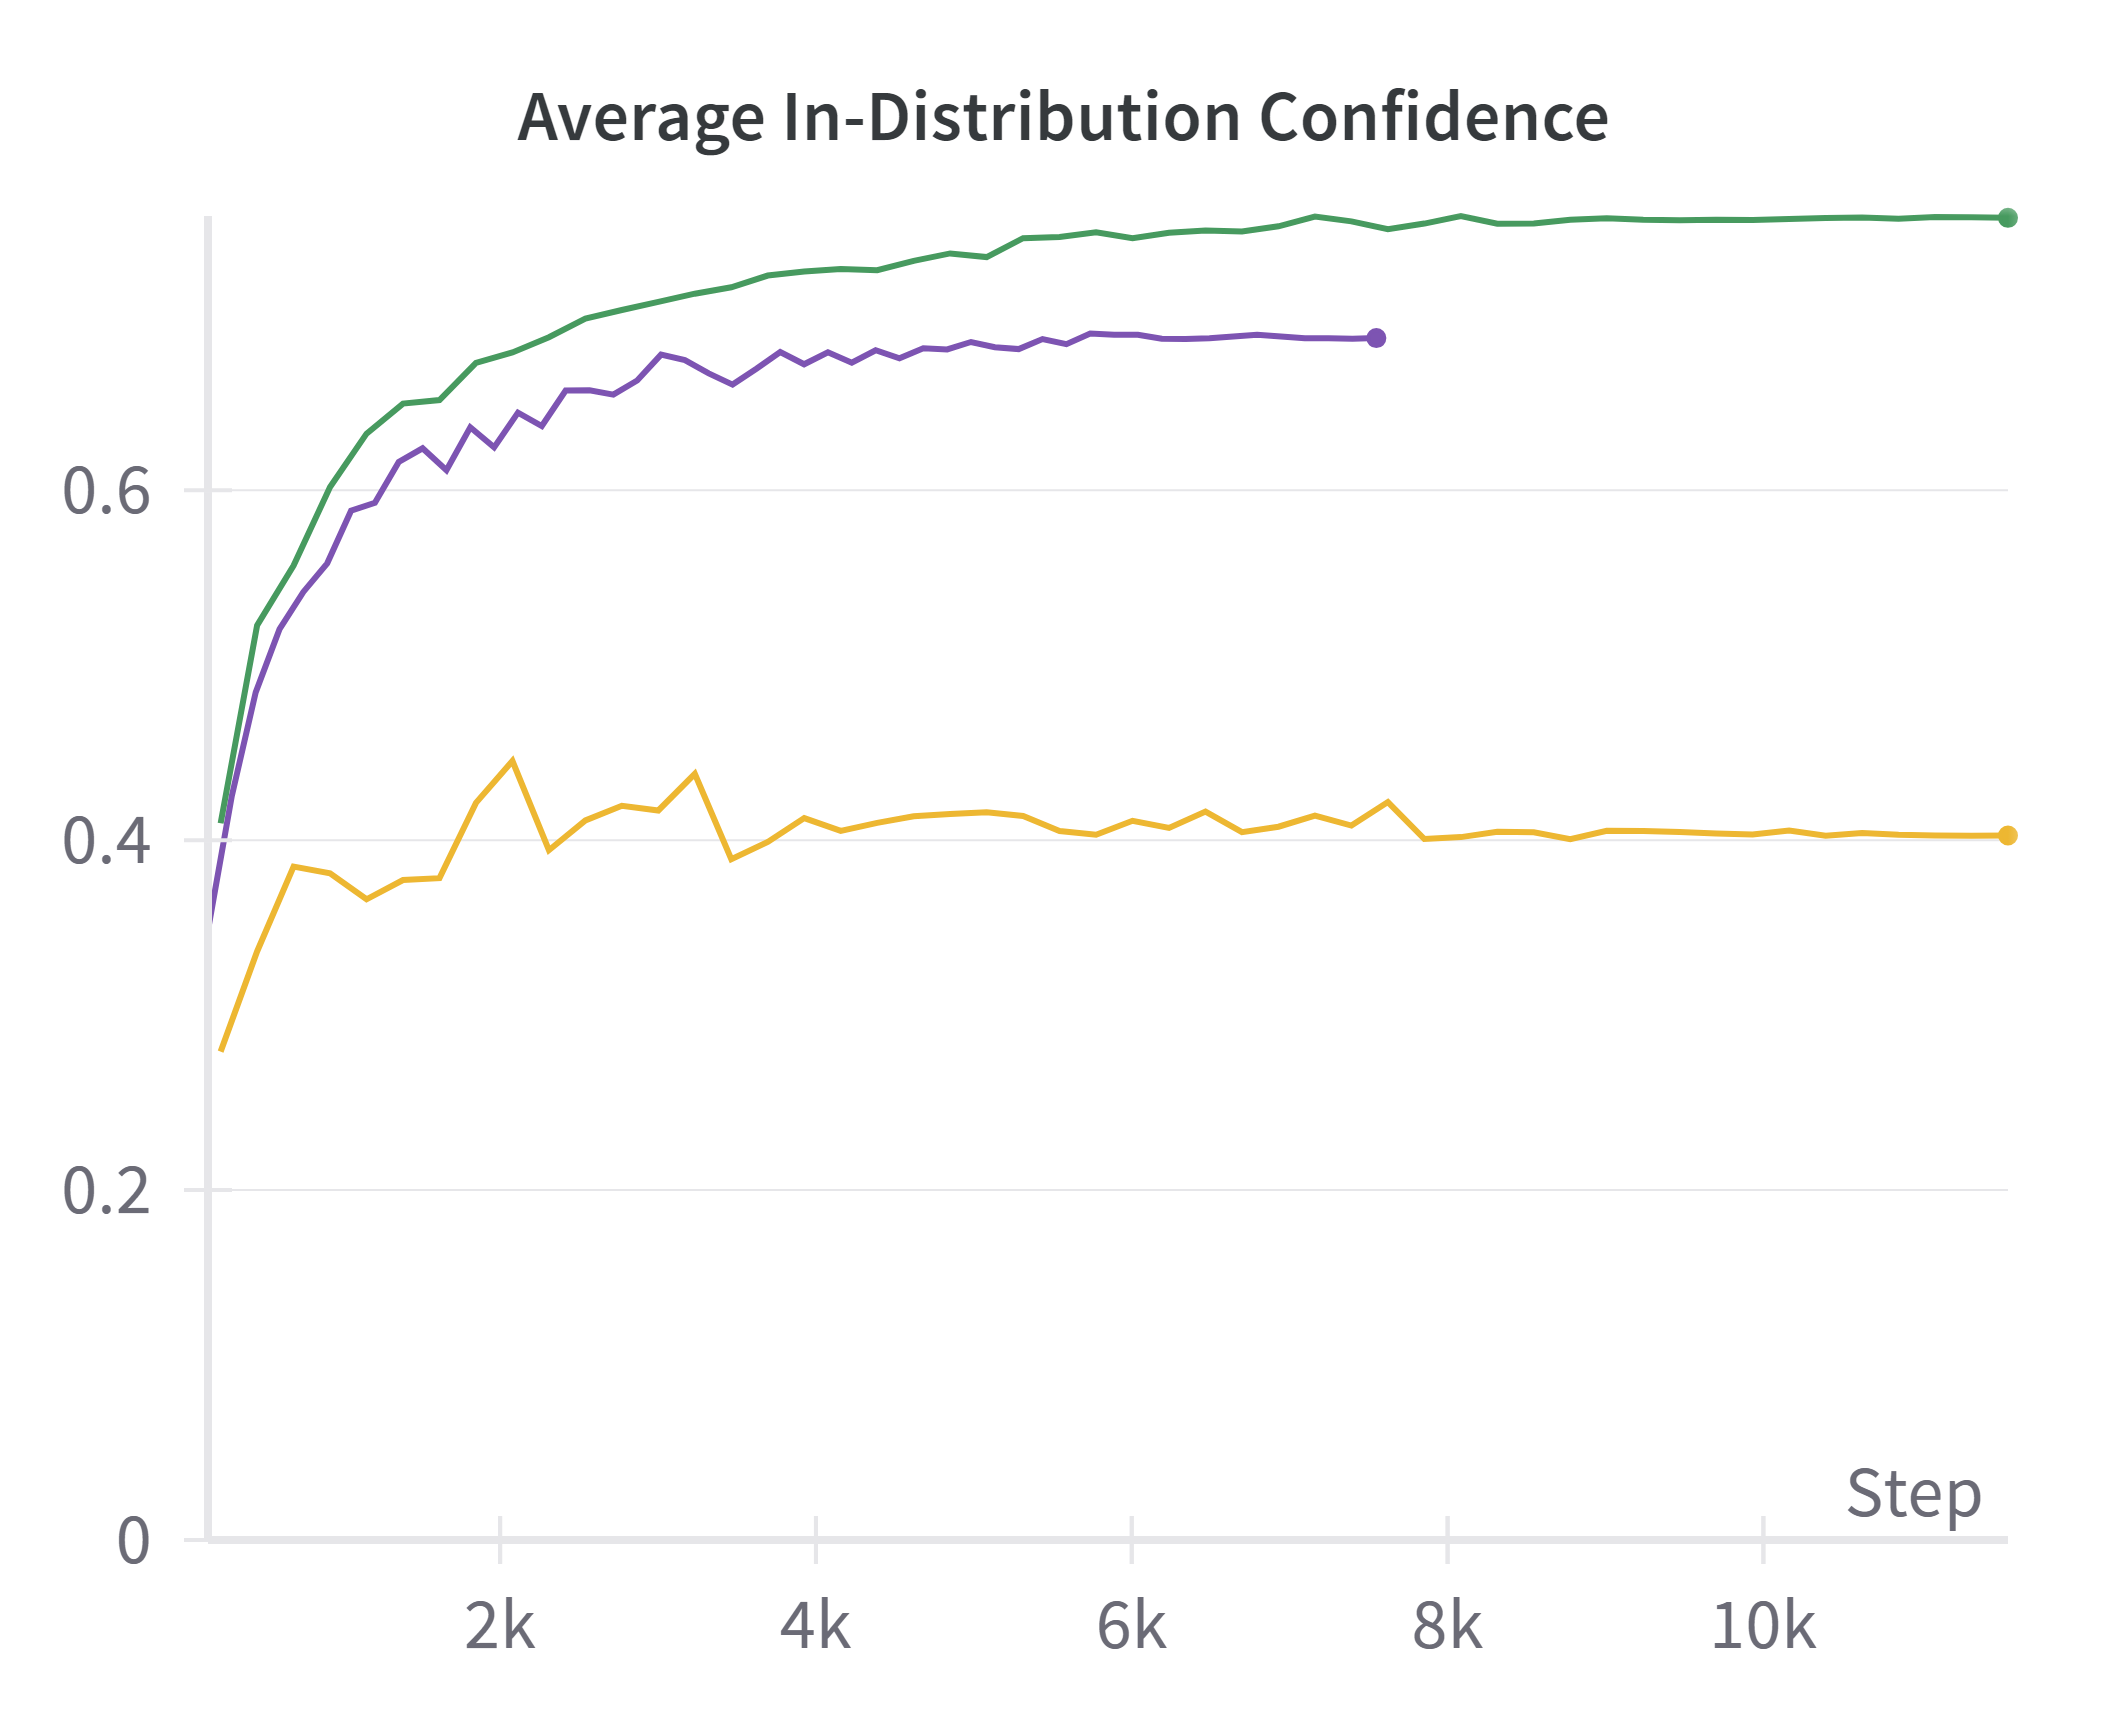
\includegraphics[width=0.5\textwidth]{figure_results_supcon-lin_avg-id-conf.png}%
	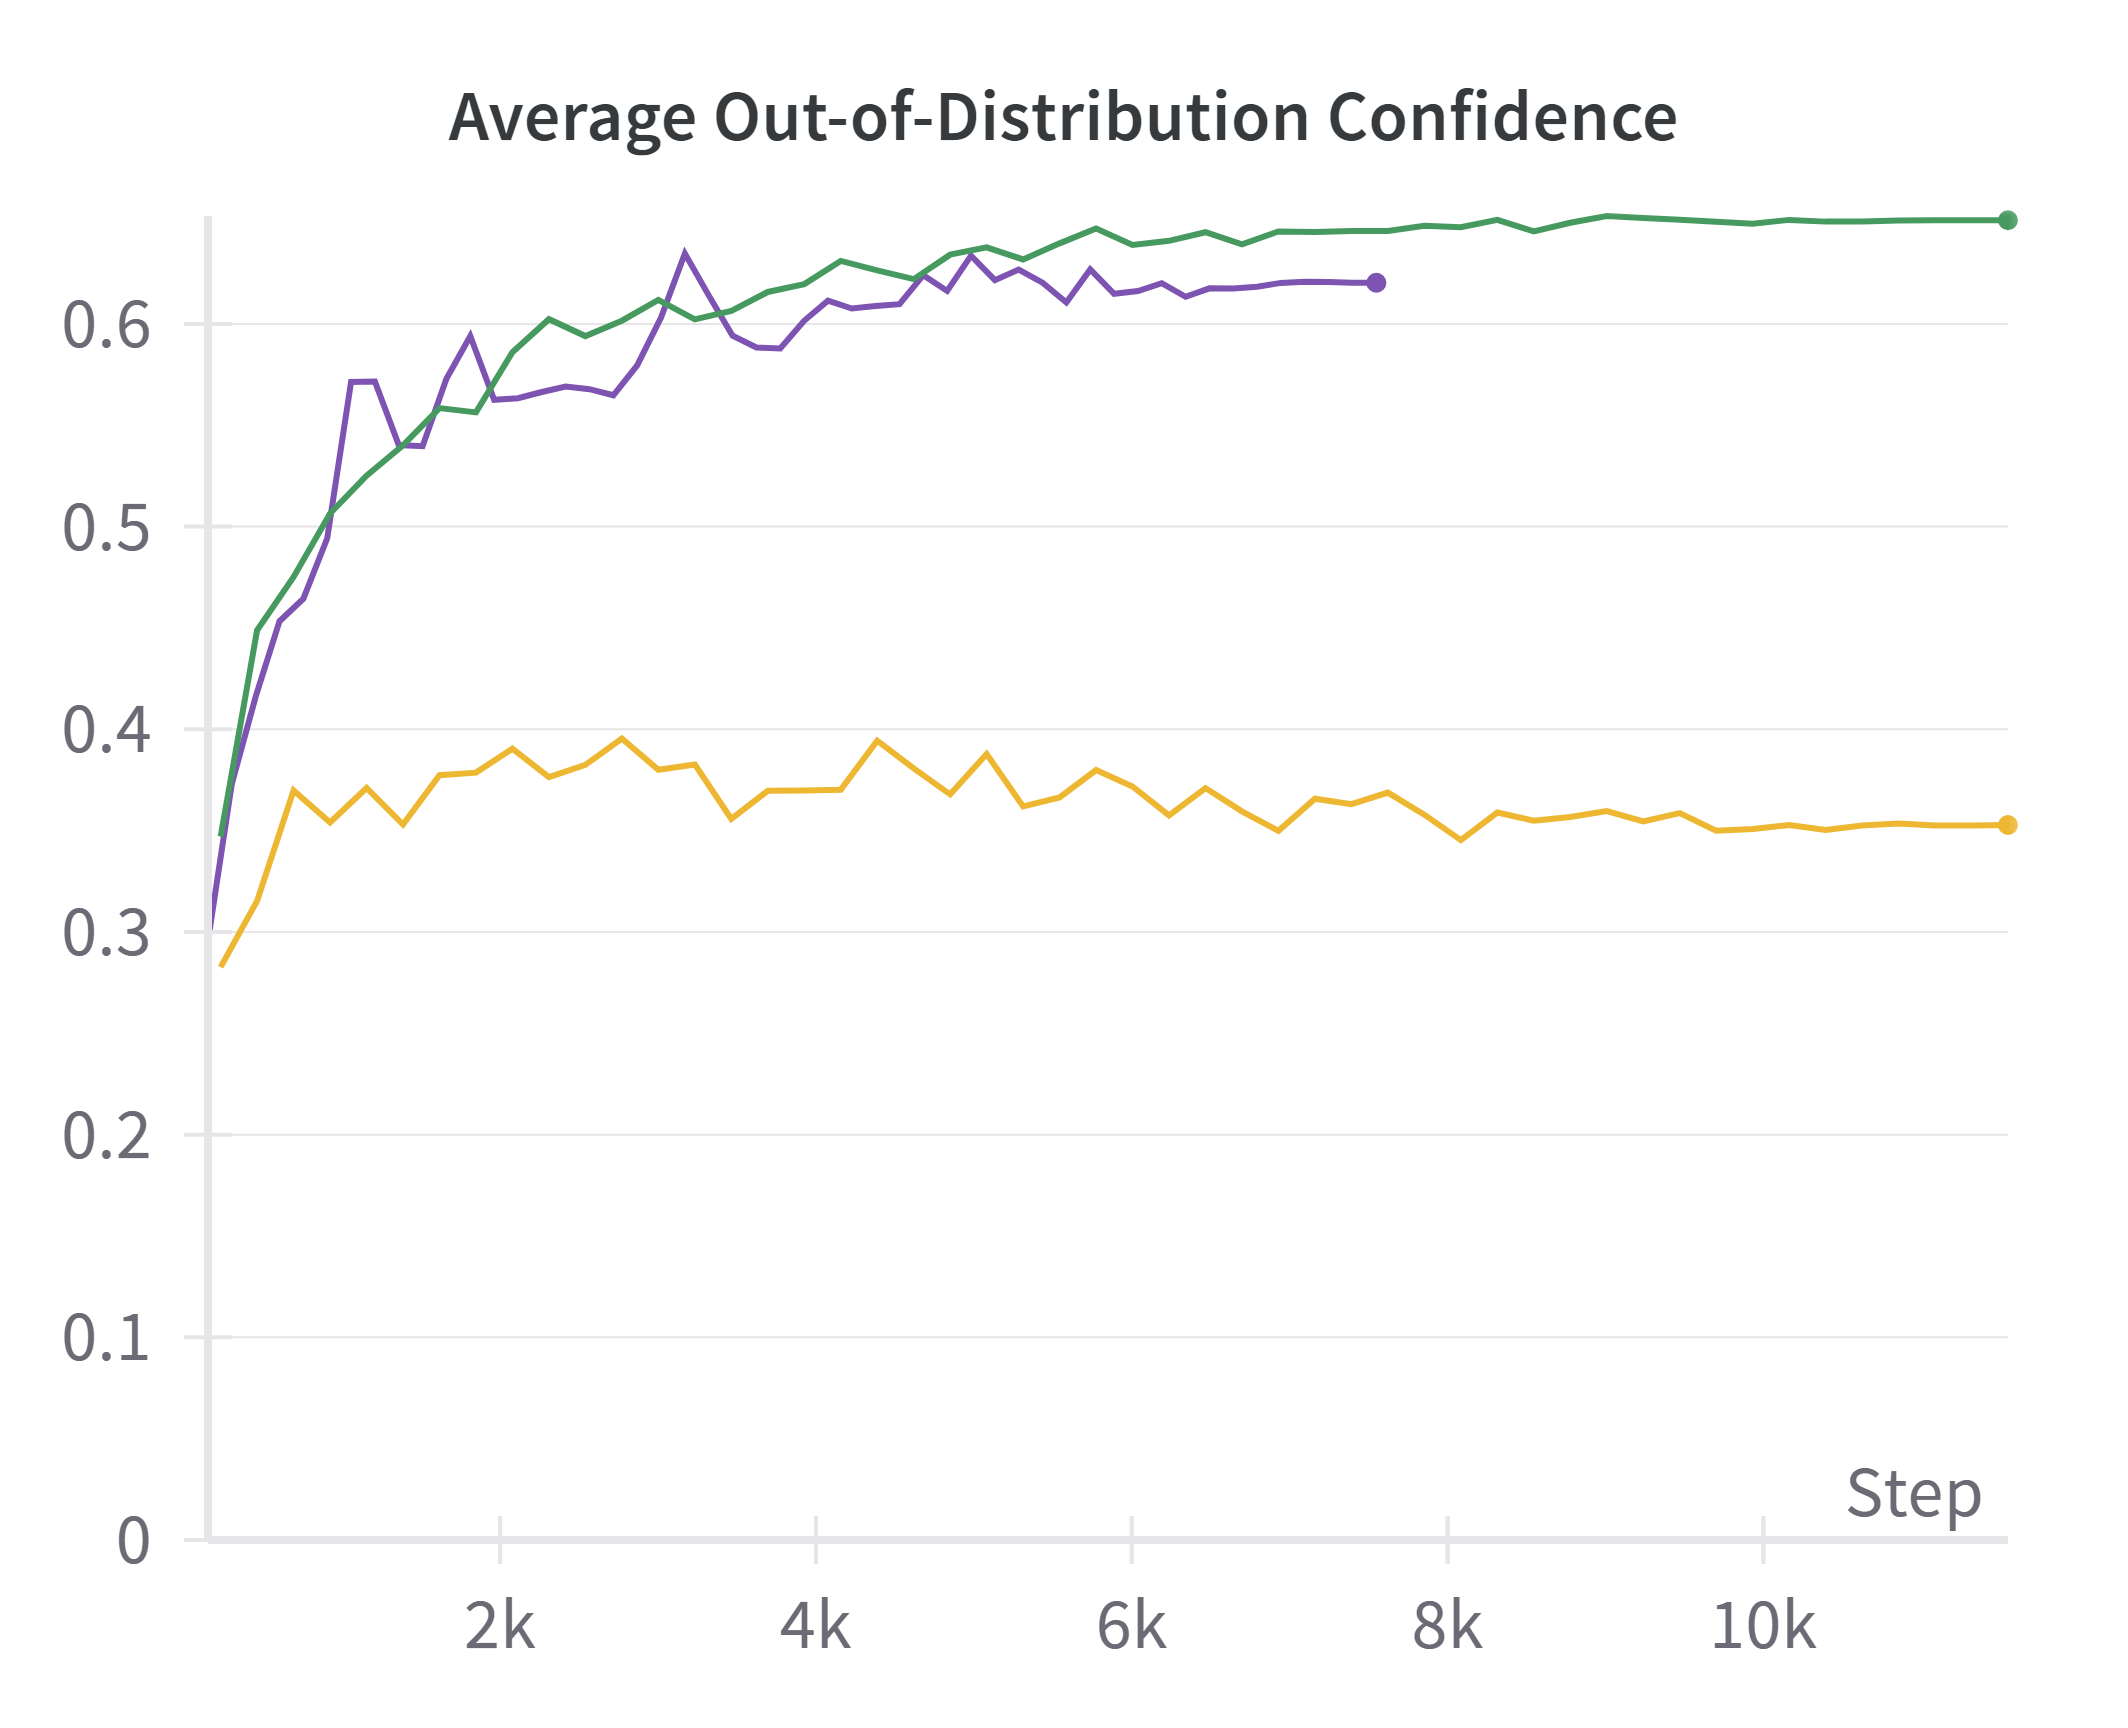
\includegraphics[width=0.5\textwidth]{figure_results_supcon-lin_avg-ood-conf.png}
	\caption[ID- und OOD-Confidence während der linearen Klassifikation.]{ID- und OOD-Confidence während der linearen Klassifikation (\textcolor{exp1}{Lila}: Versuch 1, \textcolor{exp2}{Grün}: Versuch 2, \textcolor{exp3}{Gelb}: Versuch 3).}
	\label{fig:supcon-lin-ood-detection}
\end{figure}

% Viel höherer Fehler bei Versuch 3
Die Trainingskurven der linearen Klassifikation zeigen sehr geringe Trainingsfehler für Versuch 1 und 2, aber einen viel höheren Fehler bei Versuch 3. Die Validierungsfehler der Versuche nähern sich wieder etwas an, wobei weiterhin ein deutlicer Abstand zwischen Versuch 3 und den anderen Versuchen besteht. Während der Validierungsfehler bei den Versuchen 1 und 2 also höher ist als der Trainingsfehler, ist es bei Versuch 3 umgekehrt.

% Viel geringere Trainingsgenauigkeit bei Versuch 3, dann ber doch hohe Validierungsgenauigkeit (?)
Ähnliches kann in Bezug auf die Top-1 Accuracy beobachtet werden. Die Trainingsgenauigkeit ist bei Versuch 3 deutlich niedriger als bei den anderen Versuchen, während die Validierungsgenauigkeit ein ähnlich hohes Niveau erreicht.

% Versuch 3 mit Abstand die niedrigsten Confidence-Werte (ID & OOD), und sogar den niedrigsten Abstand
Die ID-Confidence ist bei Versuch 2 deutlich höher als bei Versuch 1, während die OOD-Confidence bei beiden Versuchen vergleichbar bleibt. Versuch 3 zeigt jedoch die niedrigsten Confidence-Werte, sowohl für ID als auch für OOD, und hat auch den niedrigsten Abstand zwischen den beiden Werten. In der Trainingskurve ist dabei kaum Konvergenz zu erkennen.

In \autoref{tab:supcon-lin-results} sind die Testergebnisse der linearen Klassifikation zusammengefasst.

\begin{table}[h]
	%\centering
	\caption{Testergebnisse der linearen Klassifikation.}
	\begin{tabular}{|c|c|c|}
		\hline
		\textbf{Versuch} & \textbf{Top-1 Accuracy} & \textbf{ID-/OOD-Confidence ($\Delta$)} \\
		\hline
		1 & 71.4\% & 0.69 / 0.62 (0.07) \\
		2 & 77.5\% & 0.76 / 0.65 (0.11) \\
		3 & 75.3\% & 0.40 / 0.35 (0.05) \\
		\hline
	\end{tabular}
	\label{tab:supcon-lin-results}
\end{table}

\section{Vergleich der Ergebnisse} \label{sec:results-comparison}

% Einleitung
Als Grundlage für die Diskussion und Beantwortung der Forschungsfragen werden die Ergebnisse mit und ohne In-Distribution- und Near Out-of-Distribution-Augmentationen verglichen. Es wird auf die Klassifikations-Performance (Accuracy) und die Out-of-Distribution-Detektion (ID-/OOD-Confidence) eingegangen.

\subsection{Mit und ohne In-Distribution-Augmentationen} \label{subsec:results-comparison-id}

% Metriken
Die Klassifikations-Performance der Modelle verbesserte sich durch die In-Distribution-Augmentationen. Die Top-1 Accuracy stieg von 71.4\% auf 77.5\% und die ID-Confidence von 0.69 auf 0.76. Die OOD-Confidence stieg zwar ebenfalls von 0.62 auf 0.65, doch der Abstand zwischen ID- und OOD-Confidence wurde von 0.07 auf 0.11 angehoben.

% Verbesserung der Performance
Die Verbesserung der Performance durch die In-Distribution-Augmentationen ist auf die bessere Generalisierung der Modelle zurückzuführen. Die Modelle lernen durch die Augmentationen, die Objekte besser zu erkennen und zu klassifizieren, was sich in einer höheren Accuracy und ID-Confidence widerspiegelt. Die OOD-Confidence steigt ebenfalls, jedoch nicht so stark wie die ID-Confidence, was zu einem größeren Abstand zwischen den beiden Werten führt.

\subsection{Mit und ohne Near Out-of-Distribution-Augmentationen} \label{subsec:results-comparison-ood}

% Metriken
Die Klassifikations-Performance der Modelle verschlechterte sich durch die Near Out-of-Distribution-Augmentationen. Die Top-1 Accuracy sank von 77.5\% auf 75.3\% und die ID-Confidence von 0.76 auf 0.40. Die OOD-Confidence sank ebenfalls von 0.65 auf 0.35, wobei der Abstand zwischen ID- und OOD-Confidence von 0.11 auf 0.05 verringert wurde.

% Verschlechterung der Performance
Die Verschlechterung der Performance durch die Near Out-of-Distribution-Augmentationen ist auf die schlechtere Generalisierung der Modelle zurückzuführen. Die Modelle lernen durch die Augmentationen, die Objekte schlechter zu erkennen und zu klassifizieren, was sich in einer niedrigeren Accuracy und ID-Confidence widerspiegelt. Die OOD-Confidence sinkt ebenfalls, jedoch nicht so stark wie die ID-Confidence, was zu einem kleineren Abstand zwischen den beiden Werten führt.